\documentclass[a4paper,12pt]{book}
%% packages

\usepackage{blindtext} % needed for creating dummy text passages
%\usepackage{ngerman} % needed for German default language
\usepackage{amsmath} % needed for command eqref
\usepackage{amsthm}
\usepackage{amssymb} % needed for math fonts
\usepackage[
	colorlinks=true
	,breaklinks
	%,ngerman
	]{hyperref} % needed for creating hyperlinks in the document, the option colorlinks=true gets rid of the awful boxes, breaklinks breaks lonkg links (list of figures), and ngerman sets everything for german as default hyperlinks language
%\usepackage[hyphenbreaks]{breakurl} % ben�tigt f�r das Brechen von URLs in Literaturreferenzen, hyphenbreaks auch bei links, die �ber eine Seite gehen (mit hyphenation).
\usepackage{aliascnt}
\usepackage{xcolor}
\definecolor{c1}{rgb}{0,0,1} % blue
\definecolor{c2}{rgb}{0,0.3,0.9} % light blue
\definecolor{c3}{rgb}{0.3,0,0.9} % red blue
\hypersetup{
    linkcolor={c1}, % internal links
    citecolor={c2}, % citations
    urlcolor={c3} % external links/urls
}
%\usepackage{cite} % needed for cite
\usepackage[square,sort,comma,numbers]{natbib} % needed for cite and abbrvnat bibliography style
\usepackage[nottoc]{tocbibind} % needed for displaying bibliography and other in the table of contents
\usepackage{braket}%braketnotationpackage
\usepackage{graphicx} % needed for \includegraphics 
\usepackage{longtable} % needed for long tables over pages
\usepackage{bigstrut} % needed for the command \bigstrut
\usepackage{enumerate} % needed for some options in enumerate
\usepackage{todonotes} % needed for todos
\usepackage{makeidx} % needed for creating an index
\usepackage{array} % for tables and arrays
\makeindex

\usepackage{caption}%for image captions
\captionsetup[figure]{font=small}

\usepackage{float}%%figures forced wherever

\usepackage{indentfirst}

\usepackage[utf8]{inputenc}
\usepackage[greek,english]{babel}
\usepackage{lmodern}

\usepackage[toc,page]{appendix}

\usepackage{spverbatim}
%% page settings

\usepackage[top=2.5cm, bottom=3.5cm,left=2.5cm,right=2.5cm]{geometry} % needed for page border settings
\parindent=1.5cm % for space of first line of new text block
\sloppy % for writing with hyphenless justification (tries to)
\hyphenation{} % use hyphenation of tolerance parameters, http://www.jr-x.de/publikationen/latex/tipps/zeilenumbruch.html
\hyphenpenalty=10000
\exhyphenpenalty=10000
\usepackage{fancyhdr} % needed for head and foot options

\usepackage{setspace}
\onehalfspacing % or \doublespacing

\allowdisplaybreaks[1]

%% Theme
%\usetheme{Warsaw} % theme for slides
%\usetheme{Frankfurt}
%\usetheme{Madrid}
%\usetheme{Darmstadt}
%\usetheme{Copenhagen}
%\usetheme{Szeged}
%\usetheme{Goettingen}

%% Colors
%\usecolortheme{rose} % color for slides
%\usecolortheme{default}
%\usecolortheme{rose}
%\usecolortheme{seahorse}
%\definecolor{c1}{rgb}{0,0.7,0.6} % some green
%\definecolor{c2}{rgb}{0.9,0.9,0.9} % some gray
%% see http://www.sharelatex.com/learn/Beamer
%\setbeamercolor*{palette primary}{fg=white,bg=c1} % upper part
%\setbeamercolor*{palette secondary}{bg=c2} % left part (background)
%\setbeamercolor*{sidebar left}{fg=white,bg=c1} % left part with links
%\setbeamerfont{section number projected}{ % section numbers
%  family=\rmfamily,
%  series=\bfseries,
%  size=\normalsize
%  }
%\setbeamercolor{section number projected}{bg=c1} % color of section numbers and others (fg: Fontm, bg:Hintergrund)
%\setbeamercolor{item projected}{bg=c1}
%\setbeamercolor{itemize item}{fg=c1}
%\setbeamercolor{author in sidebar}{fg=white}
%\setbeamercolor{footlinecolor}{fg=black,bg=c2}

%% Fonts
%\usefonttheme{professionalfonts} % changes fonts

%% Foot
%\usenavigationsymbolstemplate{} % deafult controls off
%\setbeamertemplate{footline}[frame number] % slide number at the bottom
%\setbeamertemplate{footline}
%{%
%	\leavevmode%
%	\hbox{%
%	\begin{beamercolorbox}[wd=.3\paperwidth,ht=5ex,dp=1.5ex,left,leftskip=2mm]{footlinecolor}%
%		Foot information on the left over several lines
%	\end{beamercolorbox}%
%	\begin{beamercolorbox}[wd=.5\paperwidth,ht=5ex,dp=1.5ex,left,leftskip=2mm]{footlinecolor}%
%		Next foot part
%	\end{beamercolorbox}%
%	\begin{beamercolorbox}[wd=.2\paperwidth,ht=5ex,dp=1.5ex,right,rightskip=2mm]{footlinecolor}%
%		\insertframenumber{} / \inserttotalframenumber%
%	\end{beamercolorbox}%
%	}%
%	\vskip0pt%
%}
%% my macros

%% Text fomats
\newcommand{\tbi}[1]{\textbf{\textit{#1}}}

%% Math fonts
\newcommand{\bbA}{\mathbb{A}}
\newcommand{\bbB}{\mathbb{B}}
\newcommand{\bbC}{\mathbb{C}}
\newcommand{\bbD}{\mathbb{D}}
\newcommand{\bbE}{\mathbb{E}}
\newcommand{\bbF}{\mathbb{F}}
\newcommand{\bbG}{\mathbb{G}}
\newcommand{\bbH}{\mathbb{H}}
\newcommand{\bbI}{\mathbb{I}}
\newcommand{\bbJ}{\mathbb{J}}
\newcommand{\bbK}{\mathbb{K}}
\newcommand{\bbL}{\mathbb{L}}
\newcommand{\bbM}{\mathbb{M}}
\newcommand{\bbN}{\mathbb{N}}
\newcommand{\bbO}{\mathbb{O}}
\newcommand{\bbP}{\mathbb{P}}
\newcommand{\bbQ}{\mathbb{Q}}
\newcommand{\bbR}{\mathbb{R}}
\newcommand{\bbS}{\mathbb{S}}
\newcommand{\bbT}{\mathbb{T}}
\newcommand{\bbU}{\mathbb{U}}
\newcommand{\bbV}{\mathbb{V}}
\newcommand{\bbW}{\mathbb{W}}
\newcommand{\bbX}{\mathbb{X}}
\newcommand{\bbY}{\mathbb{Y}}
\newcommand{\bbZ}{\mathbb{Z}}

%%For theorems and stuff
\newtheorem*{theorem}{Theorem}
\newtheorem{definition}{Definition}
\numberwithin{definition}{section}
\newcommand{\defref}[1]{def \ref{#1}}
\newcommand{\secref}[1]{section \ref{#1}}
\newtheorem{proposition}{Proposition}
\numberwithin{proposition}{chapter}
\newcommand{\propref}[1]{prop \ref{#1}}

\newtheorem*{note}{Note}

%%renewcommands
%\renewcommand{\operatorname}[1]{\tbi{#1}}
\DeclareMathOperator{\Tr}{ \textup{\textbf{Tr}} }
\DeclareMathOperator{\diag}{ diag }
\DeclareMathOperator{\supp}{ \textup{supp}}
\begin{document}
\begin{titlepage}

\pagestyle{empty}
\title{Physical Examples of Quantum Entropies:\\ Properties, Calculations and Programmability}
\author{Stefanopoulos Dimitris}
\date{\today}

\newcommand{\HRule}{\rule{\linewidth}{0.5mm}} % Defines a new command for the horizontal lines, change thickness here

\begin{center}
 
%----------------------------------------------------------------------------------------
%	HEADING SECTIONS
%----------------------------------------------------------------------------------------

\textsc{Aristotle's University of Thessaloniki}\\[1cm]
\textsc{SubAtomic Physics and Technological Applications}\\[3.5cm] 


\includegraphics[scale=0.8]{figures/authsymbol.png}\\ % Include a department/university logo - this will require the graphicx package
%\textsc{\LargePhysical hhii}\\[0.5cm] % Major heading such as course name
%\textsc{\large Course code}\\[0.5cm] % Minor heading such as course title

%----------------------------------------------------------------------------------------
%	TITLE SECTION
%----------------------------------------------------------------------------------------

\HRule \\[0.4cm]
{\Large \bfseries Physical Examples of Quantum Entropies: Properties, Calculations and Programmability}\\[0.4cm] % Title of your document
\HRule \\[1.5cm]
 
\end{center}

\noindent
\begin{minipage}[t]{.49\textwidth}
\raggedright
\large
\emph{Supervisor:}\\
%Anastasios Petkou\\
Ioannis Antoniou
\end{minipage}% <-- Don't forget this one
%
\hfill
%
\begin{minipage}[t]{.49\textwidth}
\raggedleft
\begin{tabular}[t]{@{} r l @{}}
\large
\emph{Author:}\\
\large
Dimitris Stefanopoulos
\end{tabular}
\end{minipage}\\
\end{titlepage}

\pagestyle{plain}
\newpage
\thispagestyle{plain}

\vspace*{\fill}
\begin{center}
    \vspace{0.9cm}
    \textbf{Abstract}
\end{center}
The current master thesis is a study of quantum entropies in finite quantum systems. Specifically, we use examples of experimentally produced quantum states, to emphasize properties of the various quantum entropies while demonstrating analytic calculations and programming techniques. We start by establishing some important aspects of the spectral theorem. We discuss the modern literature regarding different definitions of entropies, focusing on von Neumann, Renyi and Tsallis entropies, quantum conditional entropies and the quantum relative entropy. Furthermore, we rewrite heuristic forms of the known definitions that have a clear algorithmic interpretation, thus simplifying the programmability of each entropy. Finally, we exploit the described techniques and emphasize properties of quantum entropies in classes of quantum systems such as pure states, mixed states, Werner states and entangled states. 
\vspace*{\fill}

\newpage
\vspace*{\fill}
\begin{center}
    \vspace{0.9cm}
\begin{otherlanguage}{greek}
\textbf{Περίληψη}
\end{otherlanguage}
\end{center}
\begin{otherlanguage}{greek}
Η παρούσα διπλωματική εργασία αφορά την μελέτη κβαντικών εντροπιών σε πεπερασμένα κβαντικά συστήματα. Ειδικότερα, χρησιμοποιούμε παραδείγματα κβαντικών συστημάτων που έχουν πραγματοποιηθεί πειραματικά, τονίζοντας ιδιότητες των διάφορων κβαντικών εντροπιών παρουσιάζοντας αναλυτικούς υπολογισμούς και προγραμματιστικές τεχνικές. Αρχικά, αναφέρουμε κάποιες απαραίτητες πτυχές του φασματικού θεωρήματος. Συζητούμε την σύγχρονη βιβλιογραφία σχετικά με τους διαφορετικούς ορισμούς κβαντικών εντροπιών επικεντρώνοντας στις εντροπίες \textlatin{Renyi, von Neumann, Tsallis}, τις δεσμευμένες κβαντικές εντροπίες και την σχετική κβαντική εντροπία. Στην συνέχεια, γραφούμε ευρετικούς ορισμούς των γνωστών ορισμών ώστε να επιδέχονται αλγοριθμικής ερμηνείας απλοποιώντας έτσι την προγραμματισιμότητα της κάθε εντροπίας. Τελικά, επιστρατεύοντας τις παραπάνω τεχνικές, τονίζουμε ιδιότητες των κβαντικών εντροπιών σε κλάσεις κβαντικών συστημάτων όπως καθαρές καταστάσεις, μεικτές καταστάσεις, καταστάσεις \textlatin{Werner} και διεμπλεγμένες καταστάσεις.
\end{otherlanguage}
\vspace*{\fill}
\tableofcontents
\chapter{Preliminaries}
\label{chap:1}
In this chapter we will discuss shortly some of the techniques and notations that we use in our endeavours. Most of this chapter can be found in basic books of Linear Algebra and Quantum Theory(\cite{nielsen2001separable},\cite{ballentine2014quantum},\cite{hall2013quantum},\cite{holevo2012quantum},\cite{wilde2013quantum}). However, we try to collect just the bare minimum needed for this thesis, in order to ease the process of understanding our conclusions.
\par
Quantum theory, as the experienced reader surely knows, is a mathematical theory that many physical models/systems must somehow obey. Its phenomenology does not appear as an inherent part of the theory(as opposed to electromagnetism or relativity) rather as an impromptu that predicts results of given experiments under some extra assumptions. Assumptions motivated by the rest of physics. For example, in quantum field theory one needs to specify a Lagrangian(i.e. type of interaction, kinematic term) and then apply the "quantum rules" in order to predict experimental results. This seemingly contentless ontology allows quantum theory to be abstract enough, hoping for applicability to pretty much any system imaginable.
\par
Why this loquacious (maybe badly received) introduction? Just to note that quantum theory can be applied to a huge collection of different physical systems and to emphasize that we will focus only on a small part of these. We will deal(mostly) with low dimensional finite quantum systems. These are systems like electron spin and photon polarization, or more generally systems that have discrete and distinct states. In the quantum mechanical language, these restrictions translate to matrices and vectors, thus, simplifying our calculations to the furthest extend(allowing us to do common linear algebra). Hence, for the rest of this thesis, unless is otherwise specified, when we are speaking of a quantum system we mean a finite and discrete one. Worth noting though, most if not all definitions and theorems that we 'll use, have a corresponding(sometimes equivalent) more general definition for infinite systems(discrete or continuous).
\section{Linear Algebra and Operators}
In quantum mechanics we represent states $\psi$ with the ket vector $\ket{\psi}$ that belongs in a d-dimensional complex Hilbert Space $\mathcal{H}$(\cite{reed1980methods}). A Hilbert space in our case can be thought of as a vector space with some inner product. There is one to one correspondence with the bra $\bra{\psi}$ that belongs to the dual space(which can be defined as a functional of the ket vector): 
$$\ket{\psi}=\left(\begin{array}{c}\psi_{1} \\ \vdots \\ \psi_{d}\end{array}\right), \qquad \bra{\psi}= \left(\begin{array}{c}\psi_{1} \\ \vdots \\ \psi_{b}\end{array}\right)^{\dagger}=\left(\psi_{1}^{*}, \ldots, \psi_{b}^{*}\right)$$
with $\dagger$ noting the adjoint. As usual we will denote the inner product with $\braket{\psi|\chi}$.
Each vector ket can be expressed with an orthonormal basis in the Hilbert space (linearly independent d-dimensional unit vectors with $\braket{e_n|e_m}=\delta_{mn}$). We will exclusively use the Standard or Natural Basis for which:
$$
\left(\begin{array}{c}
\psi_{1} \\
\vdots \\
\psi_{d}
\end{array}\right)=\sum_{\nu=1}^{d} \psi_{\nu} \ket{e_{\nu}},
\qquad
\ket{e_{1}}=\left(\begin{array}{c}
1 \\
\vdots \\
0
\end{array}\right), \ldots, \ket{e_{d}}=\left(\begin{array}{c}
0 \\
\vdots \\
1
\end{array}\right)
$$
While dealing with composite systems, we use the tensor product of the two separate Hilbert spaces in order to make our calculations for the whole system. We also need the tensor product basis(two-qubit systems):
$$
|00 \rangle=|0\rangle|0\rangle=|0\rangle \otimes |0\rangle=
\left(\begin{array}{c}
1\\
0\\
\end{array}
\right)
\otimes
\left( 
\begin{array}{c}
1\\
0\\
\end{array}
\right)=\left(\begin{array}{c}
1 \\
0\\
0\\
0\\
\end{array}\right)
$$
$$
|01 \rangle=|0\rangle|1\rangle=|0\rangle \otimes |1\rangle=
\left(\begin{array}{c}
1\\
0\\
\end{array}
\right)
\otimes
\left( 
\begin{array}{c}
0\\
1\\
\end{array}
\right)=\left(\begin{array}{c}
0 \\
1\\
0\\
0\\
\end{array}\right)
$$
$$
|10 \rangle=|1\rangle|0\rangle=|1\rangle \otimes |0\rangle=
\left(\begin{array}{c}
0\\
1\\
\end{array}
\right)
\otimes
\left( 
\begin{array}{c}
1\\
0\\
\end{array}
\right)=\left(\begin{array}{c}
0 \\
0\\
1\\
0\\
\end{array}\right)
$$
$$
|11 \rangle=|1\rangle|1\rangle=|1\rangle \otimes |1\rangle=
\left(\begin{array}{c}
0\\
1\\
\end{array}
\right)
\otimes
\left( 
\begin{array}{c}
0\\
1\\
\end{array}
\right)=\left(\begin{array}{c}
0\\
0\\
0\\
1\\
\end{array}\right)
$$
\\
\par
Let's turn to operators now. Operators
are central to quantum mechanics. They act on vectors, predict observables and rotate/transform states in the Hilbert space. In Quantum Theory we use self-adjoint operators ($A=A^{\dagger}$) that are represented by $d \times d$ square matrices thus allowing us to call them Hermitian in the usual sense. These matrices have some of the most useful properties of operators that we 'll use in our calculations: diagonalizability, real eigenvalues, linearity and so on.
\begin{note}
The support $\supp A$ of a positive operator $A$ is the span of eigenvectors of $A$ corresponding to positive eigenvalues.
\end{note}
\begin{note}
The span of a set of vectors is the set comprising all possible linear combinations of said vectors.
\end{note}
\begin{note}
A Hermitian operator $A$ is called positive, $A \geq 0,$ if $\langle\psi \mid A \psi\rangle \geq 0$ for all $\psi \in \mathcal{H}.$ The eigenvalues of a positive operator are all nonnegative: $a \geq 0$ for $a \in \operatorname{spec}(A)$ ($\operatorname{spec}(A)$ is the spectrum of $A$).
\end{note}
\begin{note}
We denote the set of all possible operators that act on $\mathcal{H}$ as $\mathcal{D}(\mathcal{H})$.
\end{note}
\noindent This structure can be formally defined as a group.\begin{note}
The eigenvectors of a Hermitian matrix constitute an orthogonal set of vectors.
\end{note}
\noindent In fact is a property found in symmetric and normal matrices.
\par
We must mention the concepts of a dyad and a dyadic(tensors of order two but with different ranks). Specifically, we ignore the formal definitions and focus on the operational forms that are thought of as outer products of a ket and a bra $|\psi\rangle\langle\phi|$. For some vectors in a Hilbert Space or its dual:$$(|\psi\rangle\langle\phi|)|\chi \rangle=|\psi\rangle(\langle\phi \mid \chi \rangle)$$
The outer product is an operator that can act on a vector. A following lemma states that:
$$
\Big( \ket{\psi} \bra{\chi} \Big) \otimes \Big( \ket{\lambda} \bra{\kappa} \Big)=\Big(\ket{\psi} \otimes \ket{\lambda}\Big) \Big(\bra{\chi} \otimes \bra{\kappa}\Big)
$$
\par
We merely mention projectors. They are an example of Hermitian operators that are expanded in a basis by the use of outer products of the basis vectors:
$$P \equiv \sum_{i=1}^{d}|i\rangle\langle i|$$
They project the vector to a subspace.
\subsection{Matrix Functions}
From linear algebra we conclude that any vector $|v\rangle$ in a Hilbert apace can be written as a linear superposition of a complete set of orthonormal vectors $\{\ket{\phi_i}\}$ of the Hilbert space(also a basis):
$$|\psi\rangle=\sum_{i} \psi_{i}\left|\phi_{i}\right\rangle$$
The sums here go up to $d$ the dimension of the space we work on.
\begin{note}
The orthonormal set
of eigenvectors of a Hermitian operator (d-dimensional hermitian matrix) is complete.
\end{note}
Immediately follows, that if $A\left|\phi_{i}\right\rangle=\alpha_{i}\left|\phi_{i}\right\rangle$ and the eigenvectors form a complete orthonormal set, then the operator can be reconstructed in a useful diagonal form in terms of its eigenvalues and eigenvectors:
$$
A=\sum_{i} \alpha_{i}\left|\phi_{i}\right\rangle\left\langle\phi_{i}\right|
$$
This is a form of the spectral decomposition of an operator and in our case is nothing more than matrix diagonalization.
One can use this diagonal representation to define a function of an operator as is usually the case in quantum theory textbooks:
$$
f(A)=\sum_{i} f\left(\alpha_{i}\right)\left|\phi_{i}\right\rangle\left\langle\phi_{i}\right|
$$
This is mentioned in the bibliography as the operator/functional calculus. In our case we will reinterpret this in the matrix formation and write:
$$
f(A)=M\left(\begin{array}{cccc}
f\left(\alpha_{1}\right) & 0 & \ldots & 0 \\
0 & f\left(\alpha_{2}\right) & \cdots & 0 \\
& \vdots  & \ddots & \vdots \\
0 & 0 & \cdots & f\left(\alpha_{d}\right)
\end{array}\right) M^{-1}
$$
where 
$$A=M\left(\begin{array}{cccc}
\alpha_{1} & 0 & \ldots & 0 \\
0 & \alpha_{2} & \cdots & 0 \\
& \vdots & \ddots & \vdots \\
0 & 0 & \cdots & \alpha_{d}
\end{array}\right)M^{-1}$$
$M$ is the modal matrix i.e. the square $d \times d$ matrix whose $i$th column is the eigenvector $v_i$ of A. Of course $M$ must be invertible and can be viewed as a similarity transformation of the diagonal eigenmatrix $D=diag(\alpha_1,\dots,\alpha_d)$. Via this method, we get to ignore the normalization of the eigenvectors since the division of the inverse matrix with $det(M)$, fixes the norm without our intervention. Also, turning to this matrix form automatically reveals powerful computational techniques.
\begin{note}
Whenever we claim that a certain real function $f:X\rightarrow Y$ takes an operator(matrix) in its argument, we merely mean a calculation of a matrix function based on the above approach.
\end{note}
\par
Let us emphasize something important here. Usually in textbooks of quantum mechanics or linear algebra, the spectral theorem for matrices is proved by expressing $f(A)$ as a Taylor sum, thus implying that $f$ must be an analytic function. However, in our case we will not just use analytic functions. The solution to this problem comes via functional analysis of bounded self-adjoint operators in which we can prove the validity of the spectral theorem (and the operational calculus) in its most general form. Details can be found in \cite{hall2013quantum},\cite{yosida1988functional},\cite{reed1980methods} and \cite{sternberg2019mathematical}. In many cases the statements of the spectral theorem and the definitions that is based on, may differ( Borel, bounded, Baire functions and so on). Some authors use normal operators to argue regarding the theorem. 
\par
In order to refer to these properties afterwards with some concreteness, we express the parts of the general spectral theorem that we will use in a nice form:
\begin{proposition}
The modal matrix approach of the spectral theorem holds for any real-valued measurable function of a $d \times d$  Hermitian matrix.
\label{spectraltheorem}
\end{proposition}
\noindent
In this proposition we could write Borel-measurable but for our purpose is somewhat redundant. In our case, functions will have arguments in $[0,1]$ ,even though sometimes we will define them for larger domains. In this case there is an even simpler and stronger proof of the spectral theorem(\citep{hall2013quantum}).

\section{Quantum Theory}
The usual approach to quantum theory is with axiomatic statements about observables, mean values and time evolution. We just mention here some aspects that are crucial in our analysis and refer the reader to the relevant literature for further exploration.
\subsection{The density matrix}
In modern quantum theory one of the most general cases of a quantum state is the density operator:
$$
\rho \equiv \sum_{i} p_{i}\left|\psi_{i}\right\rangle\left\langle\psi_{i}\right|
$$
which constitutes a statistical ensemble of pure states. Pure states are basically one dimensional projectors while mixed states have more than one non-zero $p_i$. The randomness of a quantum state expressed via the density matrix has two manifestations. Firstly, the  pure states expressed in a orthonormal basis satisfy the $l^2$ norm (\cite{ballentine2014quantum}) while the probability mass density $\{ p_i\}$ of the density matrix follows the $l^1$ norm with:
$$
\sum_{i} p_{i}=1
$$
In most cases the conditions that the density matrix must satisfy are (usually in an if and only if manner):
\begin{itemize}
\item $\Tr \rho=1$
\item $\rho=\rho^{\dagger}$
\item $\rho$ is positive
\end{itemize}
In the first condition the symbol $\Tr$ denotes the sum of the diagonal elements of the matrix $\rho$. The summation normalization of $\{p_i\}$ can follow from this first condition. Immediately
\begin{note}
If $\rho_n$ are the real eigenvalues of the density matrix then: $0 \leq \rho_{n} \leq 1$.
\end{note}
\noindent
All of the above, help us to conclude:
\begin{note}
When we calculate functions of quantum states we can be solely based on \propref{spectraltheorem}.
\end{note}
Formally the trace of a density matrix $\rho$ may be defined defined as:
$$
\Tr \rho =\sum_{i}\left\langle u_{i}|\rho| u_{i} \right\rangle
$$
where $\left\{\left|u_{j}\right\rangle\right\}$ is any orthonormal basis.
Let us remind you some properties of the trace that we exploit later:
\begin{note}
It can be proven that the trace of a density matrix is base invariant.
\end{note}
\begin{note}
It can be proven that $\Tr(ABC)=\Tr (CAB)=\Tr(BCA)$ and $\Tr(\ket{\psi}\bra{\chi})=\Tr(\braket{\chi | \psi})$.
\end{note}
\noindent
The above notes make our life easier. Since our calculations are based on traces of operator functions, we don't have to use more than one basis(sometimes none). 
We just mention here that a density matrix of a so called pure state is idempotent i.e. $\rho=\rho^2$. This is the case iff $\rho=\ket{\psi}\bra{\psi}$, when $\ket{\psi} \in \mathcal{H}$.
\subsection{Reduced density matrix and Partial Traces}
Composite systems of two substates are density matrices $\rho^{AB} \in \mathcal{D}(\mathcal{H})$ where $\mathcal{H}=\mathcal{H_A} \otimes\mathcal{H_B}$.
Let us restrict our previous notation:
\begin{note}
We denote as $\mathcal{D}(\mathcal{H})$ just the set of all density operators acting on $\mathcal{H}$.
\end{note}
To describe the subsystem $\rho^A$ 
of $\rho^{AB}$ we need to "trace out" subsystem $B$. To do that we, use the partial trace usually defined as:
$$
\rho^A=\Tr_{B}\left( \rho^{AB} \right) \equiv \sum_{i}\left(I_{A} \otimes\left\langle\left. i\right|_{B}\right) \rho^{AB}\left(I_{A} \otimes|i\rangle_{B}\right)\right.
$$
with $\ket{i}_B$ being any orthonormal basis for $\mathcal{H_B}$. The approach on partial trace that we will use is more practical. If we express $\rho^{AB}$ as the sum of tensor products in some basis $|i\rangle_{A} \otimes|j\rangle_{B}$:
$$
\Tr_B(\rho^{AB})=\Tr_B \left( \sum_{i, j, k, l} p_{ijkl}|i\rangle\left\langle\left. k\right|_{A} \otimes \mid j\right\rangle\left\langle\left. l\right|_{B}\right. \right)= \sum_{i, j, k, l} p_{ijkl} |i\rangle\left\langle\left. k\right|_{A}  \Tr \left(  |j\right\rangle\left\langle l\right|_{B} \right) 
$$
which uses the fact that:
\begin{note}
The partial trace is a linear operation.
\end{note}
\subsection{Entanglement}
A mixed state of a composite system, described by a density matrix $\rho$ acting on $\mathcal{H_{A}} \otimes \mathcal{H_{B}}$ is separable if there exist $p_{i} \geq 0,\left\{\rho_{A}^{i}\right\}$ and $\left\{\rho_{B}^{i}\right\}$ for which $\rho^{i}_A \in \mathcal{D}(\mathcal{H_A})$, $\rho^{i}_B \in \mathcal{D}(\mathcal{H_B})$
and
$$
\rho=\sum_{i} p_{i} \rho_{A}^{i} \otimes \rho_{B}^{i}
$$
where $\sum_{i} p_{i}=1$. Otherwise the state is called entangled. Entanglement is probably the most important byproduct of quantum theory. Lots and lots of discussions can take place about entanglement(\cite{horodecki2009quantum}). Entanglement measures (among them some quantum entropies) try to create sufficient and/or necessary conditions to decide whether or not a given density operator is entangled, as long as measuring the "amount" of entanglement in it.
\par 
Bell's inequalities were discovered using the EPR pair (one like \ref{rhomatrix}). Violation of these inequalities is though of as a sufficient criterion for entanglement. This means that local realism does not seem a valid physical assumption from this point of view.  
\par 
To avoid ambiguities regarding the words "local realism" we explain:
\begin{itemize}
\item The assumption that the physical properties of the system have definite values which exist independent of observation. This is sometimes known as the assumption of realism. 
\item The assumption that a measurement can be performed on system A that does not influence the result of a measurement on system B. This is sometimes known as the assumption of locality.
\end{itemize}
In a sense, local realism refers to the assumption that there exist an underlying joint probability distribution(with local hidden random variables) that can reproduce our experimental results \citep{cerf1997entropic}.
\chapter{Entropies}
\noindent
Let us here set up some motivation for our study:
\begin{itemize}
\item In most textbooks is suggested to use certain mathematically ill-defined conventions when calculating quantum entropies(for example $0\ln 0\equiv 0$). While these conventions might work operationally, is virtually impossible to use them when we automate the calculations with programming languages. Besides some automations in IBM's qiskit we couldn't find enough information regarding this issue.
\item It is not easy to find analytic calculations of entropies in the literature. In fact, we 'll see that in some cases is not clear how that calculations are meant to be completed based on the formal definitions. We use a lot of free parameters in our calculations. The reason? These parameters could be considered as "knobs" in experiments.
\item Why a physicist might care about quantum entropies? The statistical nature of entropies allows for experiments that directly  measure entropic quantities i.e. without being aware of state $\rho$(see \cite{islam2015measuring},\cite{de2020proposal}). Hence, studying entropies might help us to deduce properties of a system without explicitly prepare its specific state.
\item Why do we even talk about more than one entropy? Mathematically, more general forms of entropies might help to prove general results on given probability distributions or even describe some properties that less general formulas can't see. Physically the same thing happens. Different forms of entropy can  describe extra or different phenomena than the usual definition(for example Tsallis). Entropies can be seen as a mapping of statistical properties of some stochastic system to the real line.
\end{itemize}
\par
In the previous chapter we avoided to express our statements as theorems due to lack of rigor. In this chapter we become a bit more formalized and we use definitions to better serve our purpose.
\section{von Neumann Entropy}
\label{vonNeumannEntropysec}
\par
Entropy as a measure of probabilistic uncertainty originates in Boltzmann's work on statistical mechanics in the 1800's (see \cite{sharp2015translation}). Max Planck wrote down the definition in its current form as:
\begin{equation}
S=k \ln W
\end{equation}
with $W$ being the number of possible microstates for a given macrostate, while k is just the so called Boltzmann constant. This definition thought, regards just systems in thermodynamic equilibrium. 
\par
Gibbs redefined entropy as:
\begin{equation}
S(\rho)=-k \int \rho(x, t) \log (\rho(x, t)) d x
\label{gibbs}
\end{equation}
in which $\rho(x,t)$ is the probability density/mass function for the microstates. This is considered a more general formula since it can be meaningful in systems without equilibrium.
\par 
Is more easily seen now, how Shannon and von Neumann figured out their homonymous entropies. Shannon wrote down the entropy of a discrete probability mass function as:
\begin{equation}
\mathrm{H}(X)=-\sum_{i=1}^{n} \mathrm{P}\left(x_{i}\right) \log _{b} \mathrm{P}\left(x_{i}\right)
\label{shanon}
\end{equation}
In his famous original paper \cite{shannon1948mathematical}, Shannon extensively argues for the use of this formula to measure "uncertainty" in the theory of communication, a field which before Shannon's insights, had occupied only a small community of researchers. He established the use of entropy as a generally probabilistic entity and not just as a physical concept. Note that the Shannon entropy could be viewed as taking the integral \eqref{gibbs} with a different measure(making it a sum).
\par
From Shannon's paper we also get the joint entropy as:
\begin{equation}
H(x, y)=-\sum_{i, j} p(i, j) \log p(i, j)
\end{equation}
To turn to our primal goal, the von Neumann entropy is the generalization of the Shannon entropy in operator algebras as discussed in \cite{von2018mathematical} and then more analytically studied by Segal \citep{segal1960note}, Nakamura \citep{nakamura1961note}, and others. 
\par
\begin{definition}(Von Neumann entropy)The von Neumann entropy of a quantum state $\rho$ is defined as:
\begin{equation}
S(\rho)\equiv -\operatorname{Tr}(\rho \log \rho).
\label{vonNeumann}
\end{equation}
\end{definition}
\begin{note}The logarithms are taken to natural base. 
\end{note}
\begin{note}
This density matrix formulation of the entropy is not needed in cases of thermal equilibrium so long as the basis states are chosen to be energy eigenstates. In that case the previous definitions should be sufficient.
\end{note}
We can think of $\rho$ as probability density function when we try to get quantitative intuition. Density operators have matrix representations and is what we will mainly use in our calculations.
\begin{note}The basis of the logarithm is qualitatively irrelevant.
\end{note}
The choice of logarithm basis is nothing more than a convention.
Our main goal is for the definitions to be clearly calculatable and programmable. To do that, one of the "problems" that the above definition creates is the calculation of $0 \ln 0$. As we have said some textbooks say that by convention we "define" $0 \ln 0 \equiv 0$. This is not an arbitrary convention but a perfectly reasonable extension of the definition. However, it does not help programmability. For example,  Mathematica will through an error since it will try to calculate $0 \cdot \infty$, while Python will possibly end up calculating some number with zero.
\par
There are two easy ways to describe von Neumann entropy in order to serve our goals. We write a function that will help us re-express \ref{vonNeumann}. Let $F: \mathbb{R}^{+} \rightarrow \mathbb{R}$ in which $\mathbb{R}^{+}= \{x \geq 0|x \in \mathbb{R} \} $ as:
\begin{equation}
F(x)=\lim_{\epsilon \to x^{+}}(\epsilon \ln \epsilon).
\label{prac_von}
\end{equation}
This could work for frameworks that allow automated calculation of limits. In the case off a non-symbolic programming framework(like C or Python), $F$ should take the form:
\begin{equation}
F(x)= 
 \begin{cases} 
      0 & x=0 \\
      x \log x & x > 0 
\end{cases}
\end{equation}
as stated in \cite{holevo2012quantum}. Similar approaches can be formulated with the Iverson Bracket or some step function. The reason we define this simple function explicitly is to emphasize that this is the function that accepts the matrix generalization. These definitions help us to write down the calculations with a bit more rigor or program a function in some computer language.
\par
Following Holevo (\citep{holevo2012quantum}), Shannon entropy could now stated as:
\begin{equation}
\mathrm{H}(X)=-\sum_{i=1}^{n} F(\mathrm{P}\left(x_{i}\right))
\label{shanon2}
\end{equation}
without loss of rigor in the case of a probability zero event.
We define the von Neumann entropy in its more practical form for calculation reasons:
\begin{definition}(Heuristic von Neumann entropy)For a density matrix $\rho \in \mathcal{D}(\mathcal{H})$ the heuristic form of the von Neumann entropy is defined as:
\label{vonNeumanndef}
\begin{equation}
S(\rho)=-\Tr(F(\rho))
\label{vonNeumann2}
\end{equation}
in which F is the function $F: [0,1] \rightarrow \mathbb{R}$: 
\begin{equation}
F(x)=\lim_{\epsilon \to x}(\epsilon \log \epsilon)
\end{equation}
\end{definition}
\noindent
The domain of the function now is $[0,1]$ which has no implications in the results. 
The von Neumann entropy in a sense, measures the mixidity of a state as explain in \cite{susskind2005introduction}. This is demonstrated later in our calculations. 
\par
Using the cyclic property of the trace and the modal matrix decomposition we can simplify the above definition. We end up with the Shannon entropy of the eigenvalues $\lambda_i$ of $\rho$:
\begin{equation}
S(\rho)=-\sum_{i} F(\lambda_i)
\end{equation}
\noindent
We later write the above simplification as a general proposition based on the definitions.


\section{Renyi Entropy}
One of the widely used generalizations of Shannon entropy is the Renyi entropy. It was introduced originaly in \cite{renyi1961measures} for the probability mass  $X_k=\{p_{i}\}=\{p_{1},p_{2},....p_{k}\}$ as:
\begin{equation}
H_{\alpha}\left(X_{k}\right)=\frac{1}{1-\alpha} \log \left(\sum_{i} p_{i}^{\alpha}\right)
\end{equation}
for which $\alpha \in (0,1) \cup (1,\infty)$ is a parameter.
\par 
Using Umegaki's techniques Petz(\cite{petz1986quasi},\cite{umegaki1962conditional}) generalized Renyi entropy to it's quantum version:
\begin{definition}
(Quantum Renyi entropy)The quantum Renyi entropy of a quantum state $\rho$ is defined as:
\begin{equation}
S_{\alpha}(\rho)=\frac{1}{1-\alpha} \log \Tr\left(\rho^{\alpha}\right), \alpha \in(0,1) \cup(1, \infty)
\end{equation}
\end{definition}
As we can clearly see this entropy does not create programmably ill-defined calculations. This is because now the function that accepts the matrix generalization is just $r(\alpha;x)=x^{\alpha}$
in which $x \in \mathbb{R}$. We re-express the quantum Renyi entropy in its heuristic form making two changes. The notation, and the use of the function $r(\alpha;x)$. Before the symbol $;$ we consider free parameters of the function while after that the variable of the function.
\begin{definition}(Heuristic quantum Renyi entropy)For a density matrix $\rho \in \mathcal{D}(\mathcal{H})$ the heuristic form of the quantum Renyi entropy is defined as:
\begin{equation}
R(\alpha ; \rho)= \frac{1}{1-\alpha} \log \Tr \left(r(\alpha;\rho)\right), \alpha \in(0,1) \cup(1, \infty)
\end{equation}
in which $r$ is the function $r:[0,1] \rightarrow \mathbb{R^{+}}$:
\begin{equation}
r(\alpha;x)=x^{\alpha}
\end{equation}
\label{renyi}
\end{definition}
Having now the heuristic formula, the programmability of this entropy is clear. Note that  the domain of the function does not create a problem similar to that of the von Neumann entropy, but the definition serves a future point. 
\begin{note}
It is proven that: $\lim _{\alpha \rightarrow 1} R(\alpha;\rho)=S(\rho)$
\end{note}
\noindent
This means that the von Neumann  entropy can be viewed as a limiting case of the Renyi entropy. Worth mentioning that for $\alpha \to 0$ and $\alpha \to \infty$ the Renyi entropy converges to the Hartley entropy and the min entropy respectively.

\section{Tsallis entropy}
Tsalis entropy is another extensively used generalization  of common entropies with one parameter (see \cite{tsallis1998},\cite{tsallis2016}). It was originally 
proposed in 1988(\cite{tsallis1988original}) in its classical form as an alternative to \eqref{gibbs}. For a probability mass ${p_i}$:
\begin{equation}
S_{q}\left(p_{i}\right)=\frac{k}{q-1}\left(1-\sum_{i} p_{i}^{q}\right)
\end{equation}
It's quantum generalization was discussed firstly in \cite{tsallisquantum} and was rewritten later as:
\begin{definition}(Quantum Tsallis entropy)For a quantum state $\rho$ the quantum Tsallis entropy is defined as:
\begin{equation}
S_q(\rho)=\frac{1}{1-q}\left(\Tr \left(\rho^{q}\right)-1\right), q \in(0,1) \cup(1, \infty)
\end{equation}
\label{TsallisDEF}
\end{definition}
\noindent
We follow the same logic as we did in the Renyi case and redefine a heuristic form of the quantum Tsallis entropy:
\begin{definition}(Heuristic quantum Tsallis entropy)For a density matrix $\rho \in \mathcal{D}(\mathcal{H})$ the heuristic form of the quantum Tsallis entropy is defined as:
\begin{equation}
T(q ; \rho)= \frac{1}{1-q}\left(\Tr \left[t(q;\rho)\right]-1\right), q \in(0,1) \cup(1, \infty)
\end{equation}
in which $t$ is the function $t:[0,1] \rightarrow \mathbb{R^{+}}$:
\begin{equation}
t(q;x)=x^{q}
\end{equation}
\label{tsallis}
\end{definition}
\begin{note}
It can be proved that: $S(\rho)=\lim _{q \rightarrow 1} T(q;\rho)$.
\end{note}
\section{Quantum Conditional Entropy}
We turn back to the original Shannon paper and check the conditional entropy formula:
\begin{equation}
H(x \mid y)=-\sum_{i, j} p(i, j) \log p_{i}(j)= H(x,y)-H(y)
\end{equation}
\noindent
One of the earliest times we see a quantum analog of this type of entropy is based on the definition of the conditional density matrix $\rho_{A \mid B}$(i.e. conditional probability density function) at \citep{cerf1997negative}.

However, textbooks adopt a simpler definition of the quantum conditional entropy based purely on the von Neumann entropy(\citep{nielsen_chuang_2010}):

\begin{definition}(Conditional von Neumann Entropy)The quantum version of the conditional entropy is purely based on \defref{vonNeumanndef} and is defined as:
\begin{equation}
S(A \mid B) = S(A B)-S(B)
\label{condent}
\end{equation}
\label{defcondin}
Where $S(A B)=S(\rho^{A B})$ and
$S(B)= S\left(\Tr_{A} \rho^{A B}\right)$.
\end{definition}
\noindent
It is proven that negative conditional entropy is a sufficient criterion for entanglement. This issue is explained in \citep{cerf1997entropic} and is based on Bell's inequality.
\subsection{Extra conditional entropies} The conditional form can be extended to many types/functions of quantum entropies. In the Renyi case as defined in \citep{vollbrecht2002conditional}:
\begin{definition}(Quantum Conditional Renyi Entropy)The conditional form of the quantum Renyi entropy, for a density matrix $\rho \in \mathcal{D}(\mathcal{H})$ is defined as:
\begin{equation}
R(\alpha;A \mid B)=R(\alpha;\rho^{AB})-R(\alpha;\rho^B)
\end{equation}
\end{definition}
The Tsallis conditional case is discussed in \citep{abe2001nonadditive} and defined purely based on the conditional probability distribution of the classical case, due to non commutativity of the conditional density matrix and the marginals:
\begin{definition}(Quantum Conditional Tsallis Entropy)The conditional form of the quantum Tsallis entropy is defined as:
\begin{equation}
T(q;A \mid B)=\frac{T(q;\rho^{AB})-T(q;\rho^B)}{1+(1-q) T(q;\rho^{B})}
\end{equation}
\label{tsalcond}
\end{definition}
\section{Relative Entropy}
Relative Entropy or Kullback–Leibler divergence is a measure of the "amount" of difference that two probability distributions have with one another. It is heuristically defined as:
\begin{equation}
D(p(x) \| q(x)) \equiv \sum_{x} p(x) \log \frac{p(x)}{q(x)} \equiv-H(p(x))-\sum_{x} p(x) \log q(x).
\end{equation}
The characterization as heuristic is based on the fact that we use the conventions:$- p(x) \log 0 = \infty$ for $p(x)>0$ and $0 \log 0 \equiv 0$ in order to do calculations. This entropy was introduced in its general case(using probability measures and writing the continuous form of the formula) by Kullback and Leiber in 1951 \cite{kullback1951information}.
\par
As in the case of Shannon entropy, a similar generalization process by Umegaki allows us to define the quantum version, i.e. generalizing Relative Entropy for operator algebras( more specifically for von Neumann algebras) in \cite{umegaki1962conditional}.
\par 
According to Wilde (\citep{wilde2013quantum}):
\begin{definition}(Quantum Relative Entropy) The quantum relative entropy $D(\rho \| \sigma)$ between density operators $\rho \in \mathcal{D}(\mathcal{H})$ and $\sigma \in \mathcal{L}(\mathcal{H})$ is defined by:
\begin{equation}
D(\rho \| \sigma)= 
 \begin{cases} 
      \operatorname{Tr}[ \rho\log \rho ]-\operatorname{Tr} [ \rho \log \sigma]   & \operatorname{supp}(\rho) \subseteq \operatorname{supp}(\sigma) \\
      \infty & otherwise 
\end{cases}
\end{equation}
\end{definition}
\noindent
These types of functions(that may accept infinity as a value) are characterized as generalized. They can be define with rigor with the use of measure theory(in the quantum case using operator algebras).
\par
To ease our calculations, we can use the same techniques as in \secref{vonNeumannEntropysec} and define:
\begin{definition}(Heuristic Quantum Relative Entropy)The heuristic quantum relative entropy $Q(\rho \| \sigma)$ between the density operators $\rho$ and $\sigma$ is defined by:
\label{heuristickulback}
\begin{equation}
Q(\rho \| \sigma)= S(\rho)-\lim_{\epsilon \to -\infty} \big( \operatorname{Tr}[\rho  G(\epsilon; \sigma)] \big)
\end{equation}
in which $G: [0,1] \rightarrow \mathbb{R}$ as:
\begin{equation}
G(\epsilon;x)=
\begin{cases}
   \ln x   &   x \in (0,1] \\
   \epsilon  &   x=0
\end{cases}
\end{equation}
$\epsilon$ is a free parameter with $\epsilon \in \bbR$.
\end{definition}
\noindent
This redefinition serves our calculation and programming goals sufficiently, at least for symbolic programming.
\begin{note}
The function $G(\epsilon;x)$ satisfies the conditions needed to accept spectral matrix generalization described in \autoref{chap:1}.
\end{note}
\section{Unified discriptions}
The definition of relative and conditional entropies is an ongoing discussion in the community. There are many ways to define slightly differently the various entropies and especially relative and conditional forms. Sandwiched forms(\cite{muller2013quantum}), general entropy functions(\citep{rossignoli2010generalized}), f-Relative entropy(\cite{hayashi2016quantum}) and the conditional density operator approach are some of the existing definitions. It may be the case that different definitions are all useful since the goal is to describe certain properties of a given density matrix. We discuss a small fraction of the generalized approaches just to get an overview.
\subsection{Heuristic forms}
Let's discuss now the so called "Unified Entropy". In \cite{hu2006generalized} is defined a somewhat general entropy(2-parameter formula). Different values of the two parameters conclude to different measures including Tsallis,Renyi and von Neumann entropies.
In \cite{rathie1991unified} there is an analytic study of its classical version. Based on that paper, Hu and Ye wrote down a quantum version of the unified entropy. Make sure to review \citep{hu2006generalized} and \cite{muller2013quantum} for fullness of detail.
\begin{definition}(Quantum unified entropy)For a density operator $\rho \in \mathcal{D}(\mathcal{H})$ in a Hilbert Space $\mathcal{H}$ the unified quantum entropy is defined as:
\begin{equation}
E_{r}^{s}(\rho)=\left\{\begin{array}{lll}
[(1-r) s]^{-1}\left\{\left[\operatorname{Tr}\left(\rho^{r}\right)\right]^{s}-1\right\}, & \text { if } r \neq 1, & s \neq 0 \\
(1-r)^{-1} \log \left[\operatorname{Tr}\left(\rho^{r}\right)\right], & \text { if } r \neq 1, & s=0 \\
(1-r)^{-1}\left[\operatorname{Tr}\left(\rho^{r}\right)-1\right],
 & \text { if } r \neq 1, & s=1 \\
(r-1)^{-1}\left\{\left[\operatorname{Tr}\left(\rho^{1 / r}\right)\right]^{r}-1\right\},& \text { if } r \neq 1, & s=1 / r \\
-\operatorname{Tr}(\rho \log \rho), & \text { if } r=1
\end{array}\right.
\end{equation}
where $r>0$ and $s \in \mathcal{R}$ are real parameters.
\end{definition}
\noindent
In \citep{hu2006generalized} we can see that limiting cases of the quantum unified entropy end up to the known entropies. We use that and rewrite everything in a single formula:
\begin{definition}(Heuristic Quantum (r,s)-entropy) For a density matrix $\rho \in \mathcal{D}(\mathcal{H})$ we define the heuristic form of the quantum (r,s)-entropy as:
\begin{equation}
U(r,s;\rho)=\lim_{\epsilon \to r}\Big\{ \lim_{\lambda \to s}\big\{ [(1-\epsilon) \lambda]^{-1} \big[ [\operatorname{Tr}(\rho^{\epsilon})]^{\lambda}-1 \big] \big\}  \Big\}
\end{equation}
in which $r$ and $s$ are free parameters with $r>0$.
\end{definition}
\subsection{From quantum to classical}
Let's assume that we have a density matrix $\rho \in \mathcal{D}(\mathcal{H})$ with eigenvalues $\{ \rho_i \}$. When we calculate entropies we rewrite $\rho$ as $MDM^{-1}$ in order to apply some function $F$ and result to $MF(D)M^{-1}$. We can think of an entropy as a mapping of a distribution(quantum or not) to the real line. In our case this mapping to real line, comes with the trace operation on the matrix. This means that in any case we have to calculate $\Tr \{MF(D)M^{-1}\}$. Using the cyclic property of the trace we end up to:
\begin{equation}
\sum_i F(\rho_i)
\end{equation}
Thus for some density matrix:
\begin{note}
A quantum entropy of $\rho$ and the corresponding classical entropy of the probability mass of $\rho$'s eigenvalues $\{\rho_i\}$, are equal.
\end{note}

\chapter{Calculations}
Since our motivations are about physics and realistic future implementations, we try to connect our abstract calculations to 
example states already produced in experiments. We will also use some theoretically manufactured examples, in order to demonstrate certain properties and behaviors of our results. Some calculations will be fully detailed and in others we will just state the results.
\par 
In \ref{appendix:code} you can find portions of the Mathematica code that has been used in the following calculations. The fully general code will be uploaded on my  \href{https://github.com/jmstf94}{github}.
\section{Calculation von Neumann}
\begin{itemize}
\item
Firstly we calculate the vonNeumann entropy of a so-called maximally entangled state. As an experimental example we use the 2-qubit state:
\begin{equation}
|\psi\rangle=\frac{|H\rangle|x+\rangle-i|V\rangle|x-\rangle}{\sqrt{2}}
\label{psivon}
\end{equation}
from \cite{PhysRevLett.110.167401}. Here $\ket{H}$ and $\ket{V}$ denote the
horizontal and vertical polarization of light(first qubit) while $\ket{x\pm}$ are ground and excited states a singly charged superconductor quantum dot(second qubit). The convention is usually to denote as $\ket{0}$ the horizontal polarization and the down(minus) spin of the quantum dot. Hence the state is rewritten in the tensor product:
\begin{equation}
|\psi\rangle=\frac{|01\rangle-i|10\rangle}{\sqrt{2}}=\frac{1}{\sqrt{2}}\left(
\begin{array}{c}
 0 \\
 1\\
 -i\\
 0 \\
\end{array}
\right)
\label{pspspsps}
\end{equation}
Thus the density matrix is:
\begin{align}
\label{rhomatrix}
\rho &= \ket{\psi} \bra{\psi} \nonumber \\[0.5em]
&=\frac{1}{2}\big{(}|01\rangle-i|10\rangle\big{)}\big{(}\langle01|+i\langle10|\big{)}\\[0.5em]
&=\frac{1}{2}\left(
\begin{array}{cccc}
 0 & 0 & 0 & 0 \\
 0 & 1 & i & 0 \\
 0 & -i & 1 & 0 \\
 0 & 0 & 0 & 0 \\
\end{array}
\right)\nonumber
\end{align}
Now, we write the matrix $\rho$ using its modal matrix and the corresponding diagonal matrix. 
First we find the eigenvectors and eigenvalues  of $\rho$:
\begin{equation}
\lambda_1=1,\:  \lambda_2=0,\:  \lambda_3=0,\:  \lambda_4=0, 
\end{equation}
\begin{equation}
v_1=\left(
\begin{array}{c}
 0 \\
 i\\
 1\\
 0 \\
\end{array}
\right),
\:  v_2=\left(
\begin{array}{c}
 0 \\
 0\\
 0\\
 1 \\
\end{array}
\right),
\:  v_3= \left(
\begin{array}{c}
 0 \\
 -i\\
 1\\
 0 \\
\end{array}
\right),\:  v_4= 
\left(
\begin{array}{c}
 1 \\
 0\\
 0\\
 0 \\
\end{array}
\right)
\end{equation}
Now we readily see that the modal matrix is:
\begin{equation}
M=
\left( \begin{array}{cccc}
 0 & 0 & 0 & 1 \\
 i & 0 & -i & 0 \\
 1 & 0 & 1 & 0 \\
 0 & 1 & 0 & 0 \\
\end{array}
\right)
\end{equation}
which gives us $det(M)=2i$ and : 
\begin{equation}
M^{-1}=\frac{1}{2}
\left( \begin{array}{cccc}
 0 & -i & 1 & 0 \\
 0 & 0 & 0 & 2 \\
 0 & i & 1 & 0 \\
 2 & 0 & 0 & 0 \\
\end{array}
\right).
\end{equation}
From the modal matrices we diagonalize $\rho$:
\begin{equation}
\rho=MDM^{-1}
\end{equation}
in which:
\begin{equation}
D= \diag (1,0,0,0).
\label{diag}
\end{equation}
Now, using \propref{spectraltheorem} we apply \defref{vonNeumanndef} as prescribed, in order to calculate the von Neumann entropy:
\begin{align}
S(\rho) &= -\Tr (F(\rho))\label{functionimp:1} \\[0.5em] 
&= -\Tr (F(MDM^{-1})) \nonumber \\[0.5em]
&=-\Tr \Bigg[
M
\left( \begin{array}{cccc}
 F(1) & 0 & 0 & 0 \\
 0 & F(0) & 0 & 0 \\
 0 & 0 & F(0) & 0 \\
 0 & 0 & 0 & F(0) \\
\end{array}
\right)
M^{-1}
\Bigg]
\nonumber\\[0.5em]
&=0
\label{functionimp}
\end{align}  
The result is of course expected since the vonNeumman entropy is zero if and only if $\rho$ is a pure state.

\item
Let's calculate now the von Neumann entropy of a standard example (taken from page 504 of \citep{nielsen_chuang_2010}):
\begin{align}
\rho(s) & = s \ket{0} \bra{0} + (1-s) \ket{1} \bra{1} \\[0.5em] & =  \left(
\begin{array}{cc}
 s & 0 \\
 0 & 1-s \\
\end{array}
\right)
\label{ffrefer}
\end{align}
with $0<s<1$.
Since the density matrix is already diagonal, calculating the eigenvalues and eigenvectors becomes redundant. We directly apply \defref{vonNeumann2} and get:
\begin{align}
S(\rho(s)) &= - \Tr \left[ F(\rho(s))) \right] \\[0.5em] &=
-\Tr \bigg[ \left(
\begin{array}{cc}
 s \log (s) & 0 \\
 0 & (1-s) \log (1-s) \\[0.5em]
\end{array}
\right) \bigg] \\[0.5em]
&= -(1-s) \log (1-s)-s \log (s)
\end{align}

\begin{figure}
\begin{center}
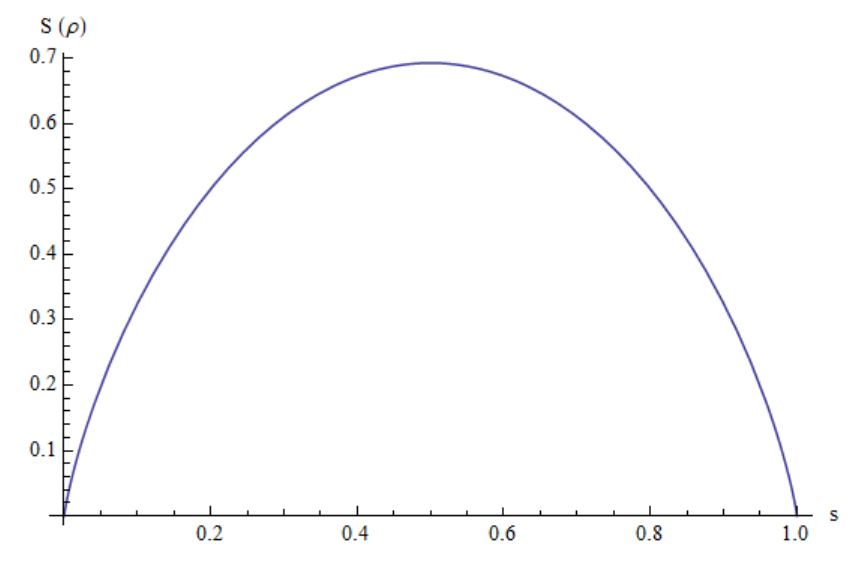
\includegraphics[scale=0.8]{figures/von_ent_plot.png}
\caption{Plotting it using the natural logarithm, demonstrates that the von Neumann entropy can measure the amount of departure from a pure state. For $s=0.5$ our state has the maximum departure from a pure state.}
\label{figure1}
\end{center}
\end{figure}

The physicality of this calculation becomes vivid, if we generalize this system to a statistical mixture of $N$ orthogonal(mutually exclusive) pure states. In the standard basis this will write:

\begin{align}
\label{asdasdas}
\rho &= \sum_{i=0}^{N-1}\rho_{i}\ket{i}\bra{i} \\[0.5em]
&= \diag (\rho_{0},\rho_{1},..,\rho_{N-2},\rho_{N-1})
\end{align}
which is an $N\times N$ diagonal matrix with \begin{equation}
\sum_{i=0}^{N-1}\rho_{i}=1
\end{equation}
Applying \defref{vonNeumanndef} we get:
\begin{align}
S(\rho) &= -\Tr \left[ \diag \big( F(\rho_{0}),F(\rho_{1}),..,F(\rho_{N-2}),F(\rho_{N-1})
 \big) \right] \\[0.5 em] &= -\sum_{i=0}^{N-1}\rho_{i} \log \rho_{i} \label{rrrrrrrrr}
\end{align}
It is easy to see the similarity with Shannon's information entropy \eqref{shanon}.
\par
Even though both information(quantum or not) and thermal entropy are generated via different methods(mathematically and conceptually), in a simple statistical mechanics problem these pure states can represent possible macrostates of a thermal system. 
\\*
For example a fixed temperature gas at a $T=1 / k_{B} \beta$ in a canonical ensemble model has a density operator:
\begin{equation}
\rho_{CE}=\frac{\exp (-\beta \hat{H})}{Z}
\end{equation}
with $\beta$ being a free parameter, $\hat{H}$ and  $\epsilon_{n}$ denotes the hamiltonian and its eigenvalues and $Z$ the quantum partition function:
\begin{equation}
Z=\Tr\left(\mathrm{e}^{-\beta \hat{H}}\right)=\sum_{i} \mathrm{e}^{-\beta \epsilon_{i}}
\end{equation}
based on the condition $\Tr(\rho)=1$. Thus each probability in \eqref{rrrrrrrrr} is:
\begin{equation}
\rho_{i}= e^{-\beta \epsilon_{i}}/Z
\end{equation}
\end{itemize}
\section{Calculation of Renyi entropy}
\begin{itemize}
\item
Now we calculate the Renyi entropy for the state $\rho$ from \eqref{rhomatrix} for an arbitrary parameter $\alpha$. The calculation process stays the same as in the case of the vonNeumann entropy, up until the function implementation at \eqref{functionimp} in which we change the function $F$ to the function $r$ adapted to \defref{renyi}:
\begin{align}
\label{functionimp1}
R(\alpha;\rho) &= \frac{1}{1-\alpha}\log \left\{ \Tr \left[ r(\alpha;\rho) \right] \right\} \\[0.5em]
&= \frac{1}{1-\alpha}\log \left\{ \Tr \left[ r(\alpha;MDM^{-1}) \right] \right\} \\[0.5em]
&=\frac{1}{1-\alpha} \log \left\{ \Tr \left[
M
\left( \begin{array}{cccc}
 1^{\alpha} & 0 & 0 & 0 \\
 0 & 0^{\alpha} & 0 & 0 \\
 0 & 0 & 0^{\alpha} & 0 \\
 0 & 0 & 0 & 0^{\alpha} \\
\end{array}
\right)
M^{-1}
\right]
\right\}
\nonumber\\[0.5em]
&=\frac{1}{1-\alpha} \log \left[ \frac{1}{2}\Tr \left(
\begin{array}{cccc}
 0 & 0 & 0 & 0 \\
 0 & 1 & i & 0 \\
 0 & -i & 1 & 0 \\
 0 & 0 & 0 & 0 \\
\end{array}
\right)
\right] \\[0.5em]
&=0
\end{align}

This is of course expected since the Renyi entropy has a minimum value of $0$ iff $\rho$ is a pure state. 
\item
Let's calculate the Renyi entropy of the diagonal density matrix $\rho$ in \eqref{ffrefer} using both $0<s<1$ and $\alpha \in(0,1) \cup(1, \infty)$ as free parameters:
\begin{align}
R(\alpha;\rho(s)) 
&= \frac{1}{1-\alpha} \log \left \{ \Tr \left[ r(\alpha;\rho(s)) \right] \right\} \\[0.5em]
&= \frac{1}{1-\alpha} \log \left\{  \Tr \left[ \left(
\begin{array}{cc}
 r(\alpha;s) & 0 \\
 0 & r(\alpha;1-s) \\[0.5em]
\end{array}
\right) \right] \right\}\\[0.5em]
&=
\frac{1}{1-\alpha} \log \left\{  \Tr \left[ \left(
\begin{array}{cc}
 s^{\alpha} & 0 \\
 0 & (1-s)^{\alpha} \\[0.5em]
\end{array}
\right) \right] \right\} \\[0.5em] 
&=\frac{1}{1-\alpha}
\log \left[ s^{\alpha }+(1-s)^{\alpha } \right]
\end{align}
Let's plot for different values of $\alpha$:
\begin{figure}[H]
\label{figure3}
\begin{center}
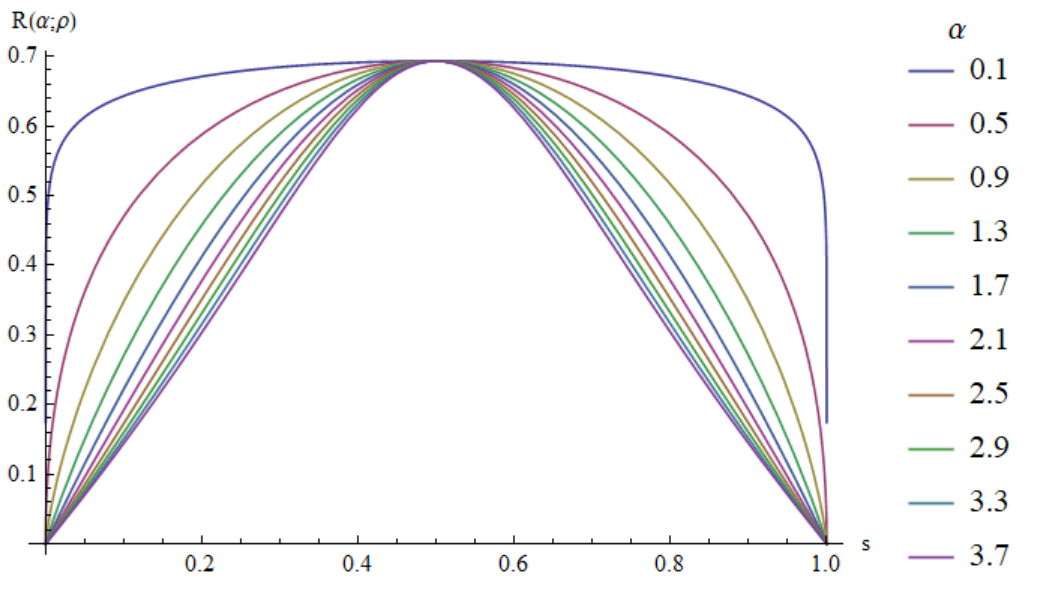
\includegraphics[scale=0.8]{figures/renyi_ent_plot.png}
\caption{Two points to make: (a)$\lim_{\alpha \to 1}R(\alpha,\rho) = S(\rho)$ is demonstrated via the similarities with figure \ref{figure1}, (b) for $s=0.5$ Renyi entropy takes the value $\log2$ independent of $\alpha$.}
\end{center}
\end{figure}
and in $3D$ for more intuition:
\begin{figure}[H]
\begin{center}
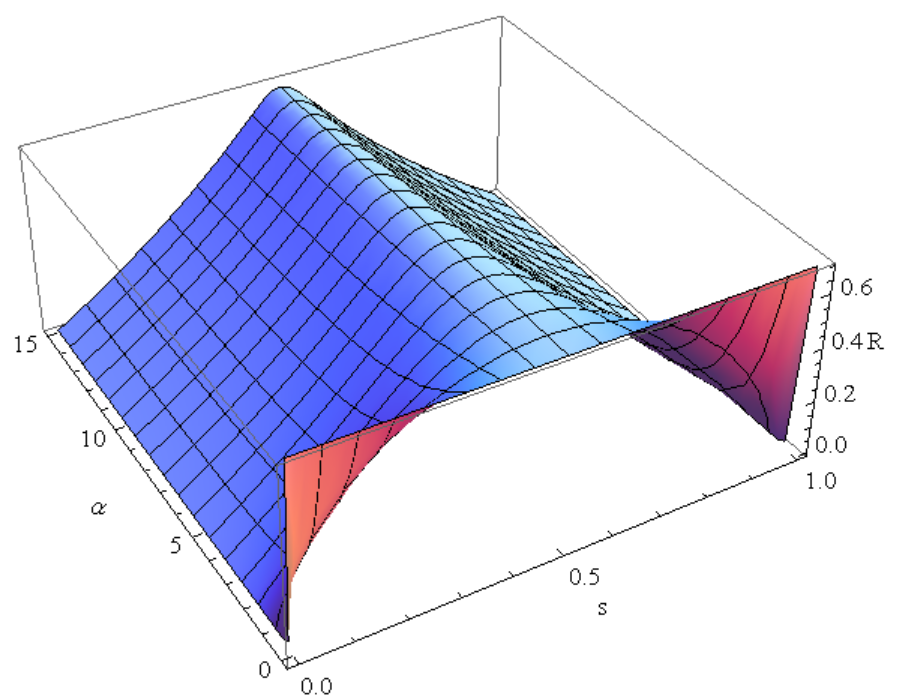
\includegraphics[scale=0.7]{figures/renyi_ent_plot_3D.png}
\caption{The 3-D plot based on the two parameters $s$ and $\alpha$.}
\label{figuridion3d}
\end{center}
\end{figure}
Regarding the example \eqref{asdasdas} the Renyi entropy is: 
\begin{align}
R(\alpha;\rho) &= \frac{1}{1-a} \log \left\{ \Tr \left[ \diag \big( r(\alpha;\rho_{0}),r(a;\rho_{1}),..,r(a;\rho_{N-2}),r(a; \rho_{N-1})
 \big) \right] \right\} \\[0.5 em] 
 &=\frac{1}{1-a} \log \left( \sum_{i=0}^{N-1}\rho_{i}^{\alpha} \right)
\end{align}
For the special case that $\rho_{i}=1/N$ we can easily see that:
\begin{equation}
R(\alpha;\rho)=\log N
\end{equation}
independent of $\alpha$.
\end{itemize}
\section{Calculation of Tsallis Entropy}
\begin{itemize}
\item
Now we calculate the Tsallis generalization of entropy for the state $\rho$ from \eqref{rhomatrix} with a parameter $q \in(0,1) \cup(1, \infty) $. The calculation process is similar to the von Neumann case, up until the function implementation at \eqref{functionimp:1} in which we change the function $F$ to the function  $t$ adapted to \defref{TsallisDEF}:
\begin{align}
\label{functionimp1}
T(q;\rho) &= \frac{1}{1-q} \left\{ \Tr \left[ t(q;\rho) \right] -1   \right\} \\[0.5em]
&= \frac{1}{1-q} \left\{ \Tr \left[ t(q;MDM^{-1}) \right] -1   \right\} \\[0.5em]
&=\frac{1}{1-q} \left\{ \Tr \left[
M
\left( \begin{array}{cccc}
 t(q;1) & 0 & 0 & 0 \\
 0 & t(q;0) & 0 & 0 \\
 0 & 0 & t(q;0) & 0 \\
 0 & 0 & 0 & t(q;0) \\
\end{array}
\right)
M^{-1}
\right]-1
\right\}
\nonumber\\[0.5em]
&=\frac{1}{1-q} \left\{ \Tr \left[
M
\left( \begin{array}{cccc}
 1^{q} & 0 & 0 & 0 \\
 0 & 0^{q} & 0 & 0 \\
 0 & 0 & 0^{q} & 0 \\
 0 & 0 & 0 & 0^{q} \\
\end{array}
\right)
M^{-1}
\right]-1
\right\}
\nonumber\\[0.5em]
&=\frac{1}{1-q} \left\{ \frac{1}{2} \Tr \left[ \left(
\begin{array}{cccc}
 0 & 0 & 0 & 0 \\
 0 & 1 & i & 0 \\
 0 & -i & 1 & 0 \\
 0 & 0 & 0 & 0 \\
\end{array}
\right) \right] -1
\right\} \\[0.5em]
&=0
\end{align}
This is of course expected since the  Tsallis entropy has a minimum value of $0$ iff $\rho$ is a pure state. 
\item
Let's calculate now the Tsallis entropy of the diagonal density matrix $\rho$ in \eqref{ffrefer} using both $0<s<1$ and $q \in(0,1) \cup(1, \infty)$ as free parameters:
\begin{align}
T(q;\rho(s)) 
&= \frac{1}{1-q} \left \{ \Tr \left[ t(q;\rho(s)) \right]-1 \right\} \\[0.5em]
&= \frac{1}{1-q} \left\{  \Tr \left[ \left(
\begin{array}{cc}
 t(q;s) & 0 \\
 0 & t(q;1-s) \\[0.5em]
\end{array}
\right) \right]-1 \right\}\\[0.5em]
&=
\frac{1}{1-q} \left\{  \Tr \left[ \left(
\begin{array}{cc}
 s^{q} & 0 \\
 0 & (1-s)^{q} \\[0.5em]
\end{array}
\right) \right]-1 \right\} \\[0.5em] 
&=\frac{\left[ s^{q }+(1-s)^{q }-1 \right]}{1-q}
\end{align}
Let's plot for different values of q:
\begin{figure}[H]
\begin{center}
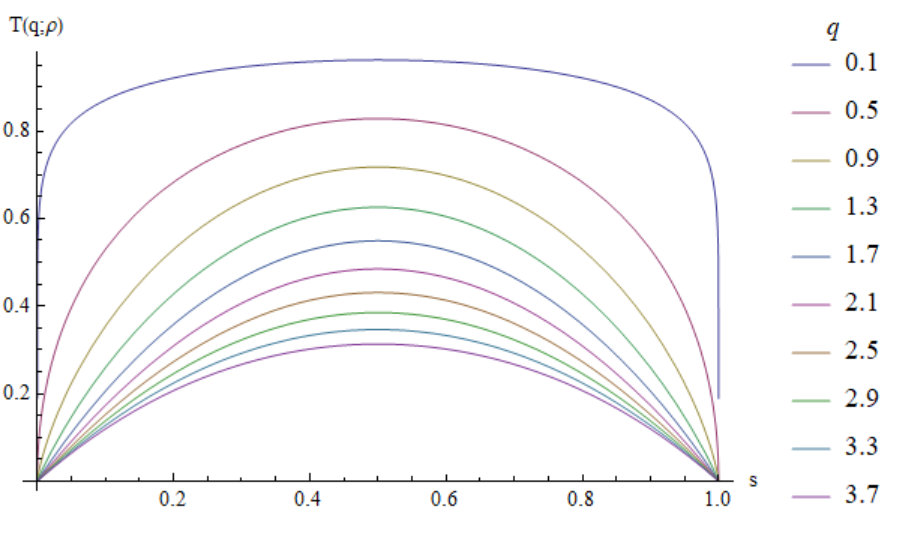
\includegraphics[scale=0.8]{figures/tsallis_ent_plot.png}
\caption{Two points to make: (a)$\lim_{q \to 1}T(q;\rho) = S(\rho)$ is demonstrated via the similarities with figure \ref{figure1}, (b) for $s=0.5$ Tsallis entropy is not independent of q.}
\end{center}
\end{figure}
and in $3D$ for more intuition:
\begin{figure}[H]
\begin{center}
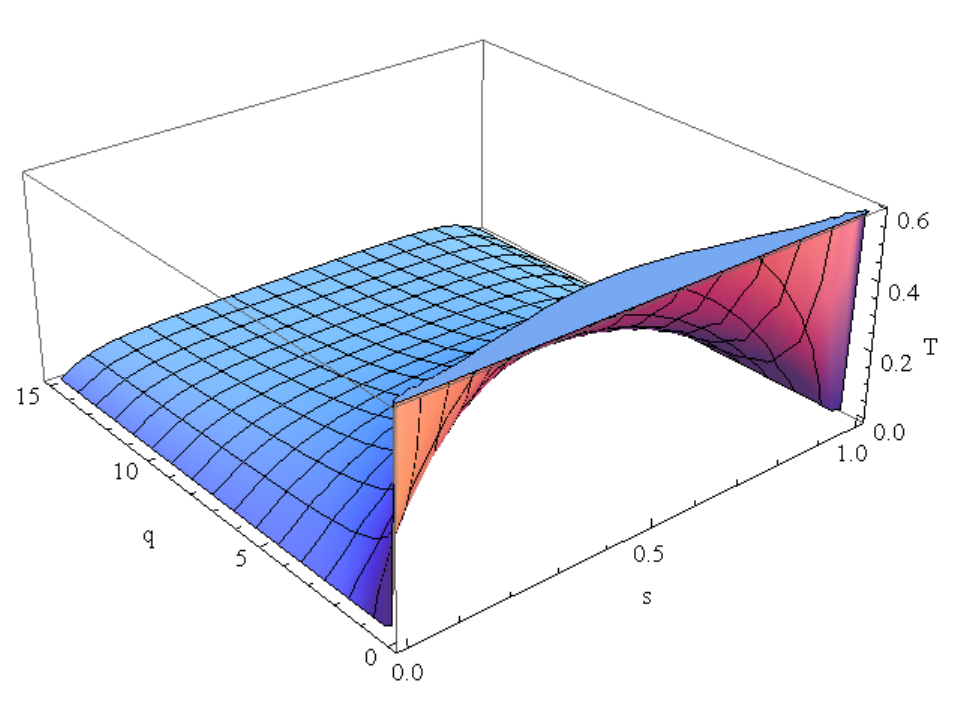
\includegraphics[scale=0.8]{figures/tsallis_ent_plot_3D.png}
\caption{The 3-D plot based on the parameters $s$ and $q$.}\label{figuridiont2}
\end{center}
\end{figure}
Regarding the example \eqref{asdasdas} for maximally mixed eigenvalues $\rho_i=N^{-1}$:
\begin{equation}
T(q;\rho)=\frac{1-N^{1-q}}{q-1}
\end{equation}
\end{itemize}

\input{parts/ConditionalEntropyCalculation}
\section{Werner State and Conditional Entropies}
Let's now take one of the most well-known and widely used states when studying conditional entropies, called Werner states. Werner, wrote down this class of states at \cite{werner1989quantum} in order to create entangled states that don't violate Bell's inequalities. Experimental demonstrations of Werner states is an active reasearch area for the last twenty years(\cite{zhang2002experimental}\cite{cinelli2004parametric}).
In our calculation we will use the theoretical form of \cite{pittenger2000note} and all the information related to its separability criteria. Specifically is noted that:
\begin{equation}
W^{\left[d^{n}\right]}(s)=(1-s) \frac{1}{d^{n}} I+s|\Psi\rangle\langle\Psi|
\label{wernerstate}
\end{equation}
where $s$ is a free parameter, $d$ is the dimension of the qudits, $n$ is the number of qudits, $\ket{\Psi}$ is an  entangled state and $I$ is the identity matrix for the composed Hilbert space. It is proven in \cite{pittenger2000note} that the state   $W^{\left[d^{n}\right]}(s)$ is fully separable if and only if $s \leq\left(1+d^{n-1}\right)^{-1}$.
We take the simplest case of $d=2$, $n=2$ and $\ket{\Psi}=(\ket{00}+\ket{11})/\sqrt{2}$ as prescribed. Thus, according to \cite{pittenger2000note} this state is separable iff $s \leq 1/3$:
\begin{align}
W &=\frac{1-s}{4}I_{4}+\frac{s}{2}(\ket{00}\bra{00}+\ket{11}\bra{11}+\ket{11}\bra{00}+\ket{00}\bra{11})\\[0.5em]&=
\left(
\begin{array}{cccc}
 (1+s)/4 & 0 & 0 & s/2 \\
 0 & (1-s)/4 & 0 & 0 \\
 0 & 0 & (1-s)/4 & 0 \\
 s/2 & 0 & 0 & (1+s)/4 \\
\end{array}
\right)
\label{wernerstate}
\end{align}
Let's calculate. Firstly, we trace out the subsystem B. It is easily done if we expand $I$ using the properties of the complete orthonormal set in standard tensor product basis(\cite{ballentine2014quantum}):
\begin{equation*}
\sum_{i}\left|\phi_{i}\right\rangle\left\langle\phi_{i}\right|=I
\end{equation*}
thus in our case:
\begin{equation*}
I_{4}=|11\rangle \langle11|+|00\rangle \langle00|+|10\rangle \langle10|+|01\rangle \langle01|
\end{equation*}
Hence:
\begin{align}
W^A &= \Tr_B (W) \nonumber \\[0.5em]
&= \Tr_B \big(\frac{1+s}{4}\ket{00}\bra{00}+\frac{1+s}{4}\ket{11}\bra{11} +\frac{1-s}{4}\ket{01}\bra{01}+\frac{1-s}{4}\ket{10}\bra{10} \nonumber \\[0.5em]&+\frac{s}{2}\ket{00}\bra{11}+\frac{s}{2}\ket{11}\bra{00} \big) \nonumber \\[0.5em]
&= \Tr_B \big(\frac{1+s}{4}|0\rangle \langle0|\otimes|0\rangle \langle0|+\frac{1+s}{4}|1\rangle \langle1|\otimes|1\rangle \langle1|  +\frac{1-s}{4}|0\rangle \langle0|\otimes|1\rangle \langle1| \nonumber \\[0.5em] &+\frac{1-s}{4}|1\rangle \langle 1|\otimes|0\rangle \langle0|+\frac{s}{2}|0\rangle \langle1|\otimes|0\rangle \langle1|+\frac{s}{2}|1\rangle \langle0|\otimes|1\rangle \langle0|
\big) \nonumber \\[0.5em]
&=\frac{1+s}{4}|0\rangle \langle0|\otimes \Tr \big( |0\rangle \langle0| \big)+\frac{1+s}{4}|1\rangle \langle1|\otimes \Tr \big( |1\rangle \langle1| \big)+\frac{1-s}{4}|0\rangle \langle0|\otimes \Tr \big(|1\rangle \langle1|\big) \nonumber \\[0.5em] &+\frac{1-s}{4}|1\rangle \langle 1|\otimes \Tr \big(|0\rangle \langle0| \big)+\frac{s}{2}|0\rangle \langle1|\otimes \Tr \big( |0\rangle \langle1| \big)+\frac{s}{2}|1\rangle \langle0|\otimes \Tr \big( |1\rangle \langle0|
\big) \nonumber \\[0.5em]
&= \frac{1+s}{4}\ket{0}\bra{0}+\frac{1+s}{4}\ket{1}\bra{1}+\frac{1-s}{4}\ket{0}\bra{0}+\frac{1-s}{4}\ket{1}\bra{1}
\nonumber \\[0.5em] &=
\frac{1}{2}\ket{0}\bra{0}+\frac{1}{2}\ket{1}\bra{1}
\nonumber \\[0.5em] &= I_{2}/2=
\left( \begin{array}{cccc}
 1/2 & 0  \\
 0 & 1/2 \\
\end{array}
\right)
\end{align}
Now let us eigen-decompose the state \eqref{wernerstate} in order to apply \propref{spectraltheorem}. We find the eigenvalues and eigenvectors of $W$:
\begin{equation}
\lambda_1=\frac{1-s}{4},\:  \lambda_2=\frac{1-s}{4},\:  \lambda_3=\frac{1-s}{4},\:  \lambda_4=\frac{1+3s}{4}, 
\end{equation}
\begin{equation}
v_1=\left(
\begin{array}{c}
 -1 \\
 0\\
 0\\
 1 \\
\end{array}
\right),
\:  v_2=\left(
\begin{array}{c}
 0 \\
 0\\
 1\\
 0 \\
\end{array}
\right),
\:  v_3= \left(
\begin{array}{c}
 0 \\
 1\\
 0\\
 0 \\
\end{array}
\right),\:  v_4= 
\left(
\begin{array}{c}
 1 \\
 0\\
 0\\
 1 \\
\end{array}
\right)
\end{equation}
Hence the modal matrix is:
\begin{equation}
M=\left(
\begin{array}{cccc}
 -1 & 0 & 0 & 1 \\
 0 & 0 & 1 & 0 \\
 0 & 1 & 0 & 0 \\
 1 & 0 & 0 & 1 \\
\end{array}
\right)
\end{equation}
which gives:
\begin{equation}
det(M)=2.
\end{equation}
As a result:
\begin{equation}
M^{-1}=
\left(
\begin{array}{cccc}
 -1/2 & 0 & 0 & 1/2 \\
 0 & 0 & 1 & 0 \\
 0 & 1 & 0 & 0 \\
 1/2 & 0 & 0 & 1/2 \\
\end{array}
\right)
\end{equation}
While the diagonal matrix:
\begin{equation}
D=\left(
\begin{array}{cccc}
(1-s)/4 & 0 & 0 & 0 \\
 0 & (1-s)/4 & 0 & 0 \\
 0 & 0 & (1-s)/4 & 0 \\
 0 & 0 & 0 & (3s+1)/4 \\
\end{array}
\right)
\end{equation}
So we have decomposed $W$ as:
\begin{equation}
W=MDM^{-1}.
\end{equation}

\subsection{von Neumann case}
\noindent
According to \eqref{condent} and \propref{spectraltheorem} we find the vonNeumann entropy for $W$ and $W^A$:
\begin{align}
S(W)&=-\Tr \big[ F(W) \big]
\nonumber \\[0.5em] &= -\Tr \big[F(MDM^{-1})\big] \nonumber \\[0.5em] &= -\Tr \left[ M
\left(
\begin{array}{cccc}
F\big((1-s)/4\big) & 0 & 0 & 0 \\
 0 & F\big((1-s)/4\big) & 0 & 0 \\
 0 & 0 & F\big((1-s)/4\big) & 0 \\
 0 & 0 & 0 & F\big((3s+1)/4\big) \\
\end{array}
\right)
M^{-1} \right]
\nonumber \\[0.5em] &=
\frac{3}{4} (s-1) \log \left(\frac{1-s}{4}\right)-\frac{1}{4} (3 s+1) \log \left(\frac{1}{4} (3 s+1)\right)
\end{align}
while:
\begin{align}
S(A)=S(W^A)&=-\Tr \big(W^A \log W^A \big) \nonumber \\[0.5em] 
&=-\Tr\left[\left( \begin{array}{cccc}
 F(1/2) & 0  \\
 0 & F(1/2) \\
\end{array}
\right) \right]
\nonumber \\[0.5em] &=-\Tr\left[\left( \begin{array}{cccc}
 -(\log 2)/2 & 0  \\
 0 & -(\log 2)/2 \\
\end{array}
\right) \right]
\nonumber \\[0.5em] &= \log2
\end{align}
Hence the conditional entropy is:
\begin{align}
S(B|A)_{W}&=S(AB)-S(A)
\nonumber \\[0.5em] &= S(W)-S(W^A)
\nonumber \\[0.5em] &= 
\frac{3}{4} (s-1) \log \left(\frac{1-s}{4}\right)-\frac{1}{4} (3 s+1) \log \left(\frac{1}{4} (3 s+1)\right)-\log (2)
\end{align}
Let's plot:
\begin{figure}[H]
\label{figure2}
\begin{center}
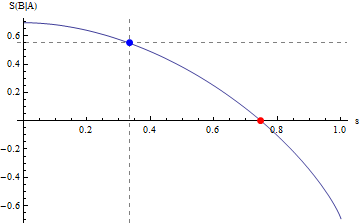
\includegraphics[scale=0.8]{figures/conditional_vonNeumann_Werner.png}
\caption{The blue point $B$ has the coordinates $(1/3,0.549306)$ and the red point $R(0.747614,0)$ which was found via numerical methods. The diagram clearly illustrates that the state $W$ while entangled($s\geq 1/3 $) has positive quantum conditional entropy, a fact emphasized by many sources(for example at \cite{nielsen2001separable}). This particular example becomes negative for $s  \gtrsim 0.747614$. A similar diagram can be found in \cite{patro2017non}.}
\end{center}
\end{figure}
\subsection{Tsallis case}
\noindent
The Tsallis entropy for the whole state as defined:
\begin{align}
T(q;W) &= \frac{1}{1-q} \left\{ \Tr \left[ t(q;W) \right] -1   \right\} \nonumber \\[0.5em]
&= \frac{1}{1-q} \left\{ \Tr \left[ t(q;MDM^{-1}) \right] -1   \right\} \nonumber \\[0.5em]
&=\frac{1}{1-q} \left\{ \Tr \left[
M
\left( \begin{array}{cccc}
 t(q;\frac{1-s}{4}) & 0 & 0 & 0 \\
 0 & t(q;\frac{1-s}{4}) & 0 & 0 \\
 0 & 0 & t(q;\frac{1-s}{4}) & 0 \\
 0 & 0 & 0 & t(q;\frac{3s+1}{4}) \\
\end{array}
\right)
M^{-1}
\right]-1
\right\}
\nonumber\\[0.5em]
&=\frac{2^{-2 q} (1-s)^q+2^{1-2 q} (1-s)^q+2^{-2 q} (3 s+1)^q-1}{1-q}.
\end{align}
For the subsystem A we readily see that:
\begin{align}
T(q;W^A)&= \frac{1}{1-q} \left\{ \Tr \left[ t(q;W^A) \right] -1   \right\} \nonumber \\[0.5em] &= \frac{2^{1-q}-1}{1-q}
\end{align}
From  the quantum conditional Tsallis entropy gives:
\begin{align}
T(B|A)_{W}&=\frac{T(q;W)-T(q;W^A)}{1+(1-q) T(q;W^A)}
\nonumber \\[0.5em] &= \frac{2^{-q-1} \left(-3 (1-s)^q-(3 s+1)^q+2^{q+1}\right)}{q-1}
\label{calccondtsa}
\end{align}
Let's plot for some values of $q$:
\begin{figure}[H]
\label{figure2}
\begin{center}
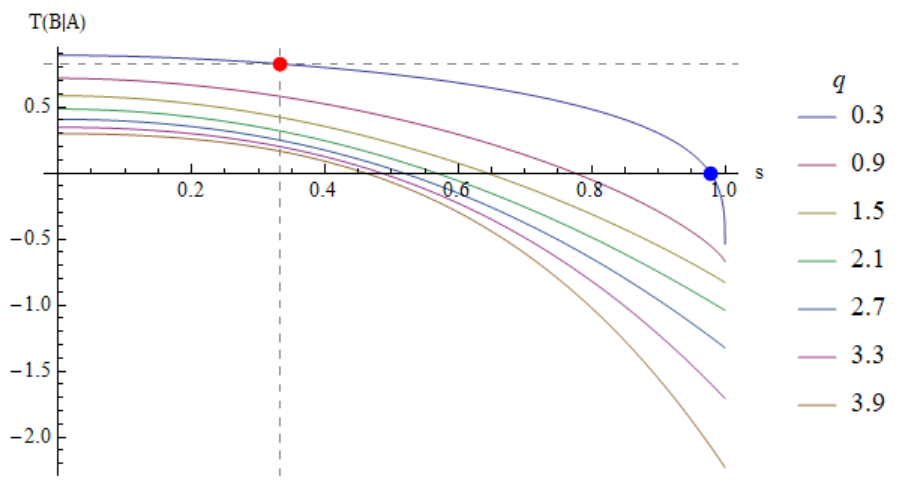
\includegraphics[scale=0.8]{figures/conditional_tsallis_werner.png}
\caption{As an example, blue point $B$ has the coordinates $(0,0.978043)$ and the red point $R(1/3,0.826907)$ which was found via numerical methods. This diagramm again illustrates that the state $W$ while entangled($s\geq 1/3 $) has positive quantum Tsallis conditional entropy for most $q$'s.}
\end{center}
\end{figure}
Let's see how the entanglement limit value of the quantum conditional Tsallis entropy changes with $q$, i.e. the value of $T(B|A)_{W}$ for $s=1/3$. From \eqref{calccondtsa} we get:
\begin{equation}
T(\tfrac{1}{3};B|A)_W= \frac{2^{-q-1} \left(-2^q+2^{q+1}-2^q 3^{1-q}\right)}{q-1}
\end{equation}
and the plot:
\begin{figure}[H]
\label{figure2}
\begin{center}
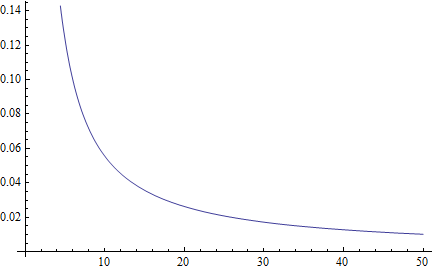
\includegraphics[scale=0.7]{figures/diag1.png}
\caption{We can numerically see in this example that for larger $q$ the entanglement limit value is getting smaller.}\label{figr1}
\end{center}
\end{figure}
\noindent
As always we present the 3Dplot for intuition:
\begin{figure}[H]
\label{figure2}
\begin{center}
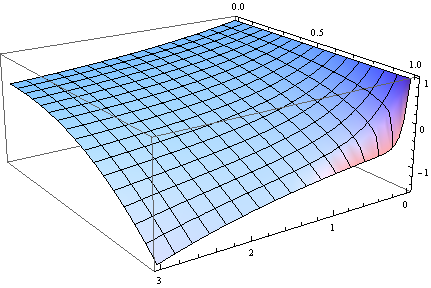
\includegraphics[scale=0.8]{figures/3DplotTsallis.png}\caption{The 3D plot of \eqref{calccondtsa}}
\label{figr2}
\end{center}
\end{figure}
\subsection{Renyi Case}
\noindent
For the total W state we find:
\begin{align}
R(\alpha;W) &= \frac{1}{1-\alpha}\log \left\{ \Tr \left[ r(\alpha;MDM^{-1}) \right] \right\} \nonumber \\[0.5em]
&=\frac{1}{1-\alpha} \log \left\{ \Tr \left[
M
\left(
\begin{array}{cccc}
 4^{-\alpha } (1-s)^{\alpha } & 0 & 0 & 0 \\
 0 & 4^{-\alpha } (1-s)^{\alpha } & 0 & 0 \\
 0 & 0 & 4^{-\alpha } (1-s)^{\alpha } & 0 \\
 0 & 0 & 0 & 4^{-\alpha } (3 s+1)^{\alpha } \\
\end{array}
\right)
M^{-1}
\right] \right\}
\nonumber\\[0.5em]
&=-\frac{\log \left(4^{-\alpha } \left(3 (1-s)^{\alpha }+(3 s+1)^{\alpha }\right)\right)}{a-1}
\end{align}
while for the subsystem:
\begin{align}
R(\alpha;W^A)&= \frac{1}{1-\alpha} \left\{\log \Tr \left[ \left(
\begin{array}{cc}
 2^{-\alpha } & 0 \\
 0 & 2^{-\alpha } \\
\end{array}
\right) \right] \right\} \nonumber \\[0.5em] &= \frac{2^{1-q}-1}{1-q}  \\[0.5em] &=
\frac{\log \left(2^{1-\alpha }\right)}{1-a}
\end{align}
Hence:
\begin{align}
R(B|A)_{W}&=R(\alpha;W)-R(\alpha;W^{A})
\nonumber \\[0.5em] &=
\frac{\log \left(2^{1-\alpha }\right)-\log \left(4^{-\alpha } \left(3 (1-s)^{\alpha }+(3 s+1)^{\alpha }\right)\right)}{\alpha -1}
\label{renyicasecalc}
\end{align}
Let's plot:
\begin{figure}[H]
\label{figure2}
\begin{center}
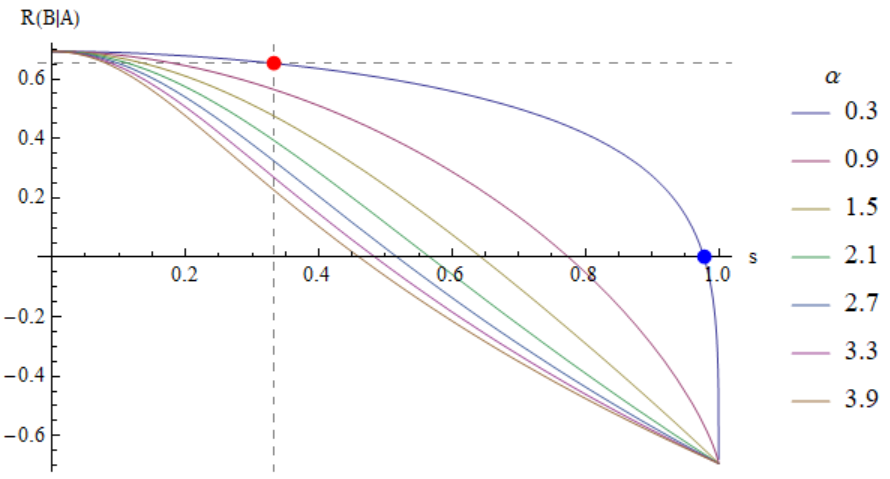
\includegraphics[scale=0.8]{figures/conditional_renyi_werner.png}
\caption{As an example, blue point $B$ has the coordinates $(0,0.978043)$ and the red point $R(1/3,0.65241)$ which was found via numerical methods. This plot again illustrates that the state $W$ while entangled($s\geq 1/3 $) has positive quantum Renyi conditional entropy for most $\alpha$'s.}
\end{center}
\end{figure}
We emphasize, that the identical value of $s$ when Tsallis and Renyi entropies are taken to zero for $\alpha=q=0.3$, is not an accident nor a mistake. It is an example of a general result $T(x ; B \mid A)_{\rho} \geq 0 \quad \Leftrightarrow \quad S(x; B \mid A)_{\rho} \geq 0$ as discussed in \cite{vollbrecht2002conditional}. As with the Tsallis entropy we the entanglement limit value for the quantum conditional Renyi entropy:
\begin{equation}
R(\tfrac{1}{3};B|A)_W=
\frac{\log \left(2^{1-\alpha }\right)-\log \left(4^{-\alpha } \left(2^{\alpha }+2^{\alpha } 3^{1-\alpha }\right)\right)}{\alpha -1}
\end{equation}
and the plot:
\begin{figure}[H]
\begin{center}
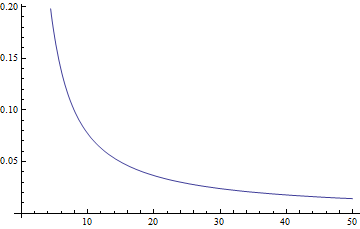
\includegraphics[scale=0.8]{figures/diag2.png}
\caption{We can numerically see in this example that for larger $\alpha$ the entanglement limit value is getting smaller.}
\label{figr3}
\end{center}
\end{figure}
\noindent
The 3-D plot will give:
\begin{figure}[H]
\begin{center}
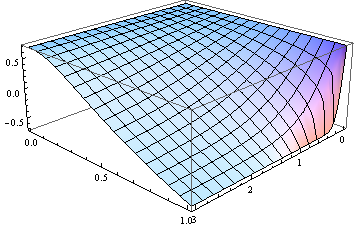
\includegraphics[scale=0.9]{figures/3DplotRenyi.png}
\caption{The 3-D plot of \eqref{renyicasecalc}}
\label{figr4}
\end{center}
\end{figure}
\section{Calculation of Relative Entropy}
\subsection{Pure-Pure}
We calculate now the quantum relative entropy of two states of the type \eqref{condentpsi} to make a somewhat general calculation with arbitrary parameters. Let the parameters be $0<u,v<\pi/2$,
hence the density matrices are $\sigma_u=\ket{\psi(u)}\bra{\psi(u)}$ and $\sigma_v=\ket{\psi(v)}\bra{\psi(v)}$. The eigendecomposition is identical to the calculation of section \ref{sectioncondcalc} thus we have all the expressions needed for our calculations.
We will calculate $Q(\sigma_u \| \sigma_v)$ but it is obviously symmetric under the interchange of variables $u$ and $v$. 

\begin{align}
Q(\sigma_u \| \sigma_v) &=S(\sigma_u)-\lim_{\epsilon \to -\infty} \left\{ \Tr \left[
\sigma_u M_v
\left(
\begin{array}{cccc}
 G(\epsilon;1) & 0 & 0 & 0 \\
 0 &  G(\epsilon;0) & 0 & 0 \\
 0 & 0 &  G(\epsilon;0) & 0 \\
 0 & 0 & 0 &  G(\epsilon;0) \\
\end{array}
\right) M_v^{-1} \right] \right\} \nonumber \\[0.5em]
&= -\lim_{\epsilon \to -\infty} \left\{ \Tr \left[ \sigma_u
\left(
\begin{array}{cccc}
 \epsilon  \sin ^2(v) & 0 & 0 & -\epsilon  \cos (v) \sin (v) \\
 0 & \epsilon  & 0 & 0 \\
 0 & 0 & \epsilon  & 0 \\
 -\epsilon  \cos (v) \sin (v) & 0 & 0 & \epsilon  \cos ^2(v) \\
\end{array}
\right)
 \right] \right\} \nonumber \\[0.5em]
&=-\lim_{\epsilon \to -\infty} \left( \epsilon  \sin ^2(v-u) \right) \nonumber \\[0.5em]
&=
\begin{cases}
   +\infty   &   u \neq v\\
   0  &   u=v
\end{cases}
\end{align}
This result is expected. Different pure states diverge while quantum relative entropy is zero the matrix arguments are identical.
\subsection{Mixed-Mixed}
We now calculate an example of a mixed vs mixed state. One is the maximally mixed state and the other is the Werner state with $\ket{\Psi}$ being the one from \eqref{wernerstate}. We calculate:
\begin{equation}
W=\left(
\begin{array}{cccc}
 (1-s)/4 & 0 & 0 & 0 \\
 0 & (s+1)/4 & is/2 & 0 \\
 0 & -is/2 & (s+1)/4 & 0 \\
 0 & 0 & 0 & (1-s)/4 \\
\end{array}
\right)
\end{equation}
vs
$I_4$.
We just state the eigendecomposition of W since the methodology is already demonstrated:
\begin{equation*}
\left(
\begin{array}{cccc}
 0 & 0 & 1 & 0 \\
 0 & -i & 0 & i \\
 0 & 1 & 0 & 1 \\
 1 & 0 & 0 & 0 \\
\end{array}
\right)
\left(
\begin{array}{cccc}
 (1-s)/4 & 0 & 0 & 0 \\
 0 & (1-s)/4 & 0 & 0 \\
 0 & 0 & (1-s)/4 & 0 \\
 0 & 0 & 0 & (3 s+1)/4 \\
\end{array}
\right)
\left(
\begin{array}{cccc}
 0 & 0 & 0 & 1 \\
 0 & \frac{i}{2} & \frac{1}{2} & 0 \\
 1 & 0 & 0 & 0 \\
 0 & -\frac{i}{2} & \frac{1}{2} & 0 \\
\end{array}
\right)
\end{equation*}
In the case  of $Q(W \| I_4)$ is readily obvious that the $\epsilon$ of the second term is absent(diagonals different from zero).
After carrying techniques  identical to sections... we find:
\begin{equation}
Q(W\|I_4)= \frac{1}{4} ((3 s+1) \log (3 s+1)-3 (s-1) \log (1-s))
\label{hjreherjrie}
\end{equation}
with the plot:
\begin{figure}[h]
\begin{center}
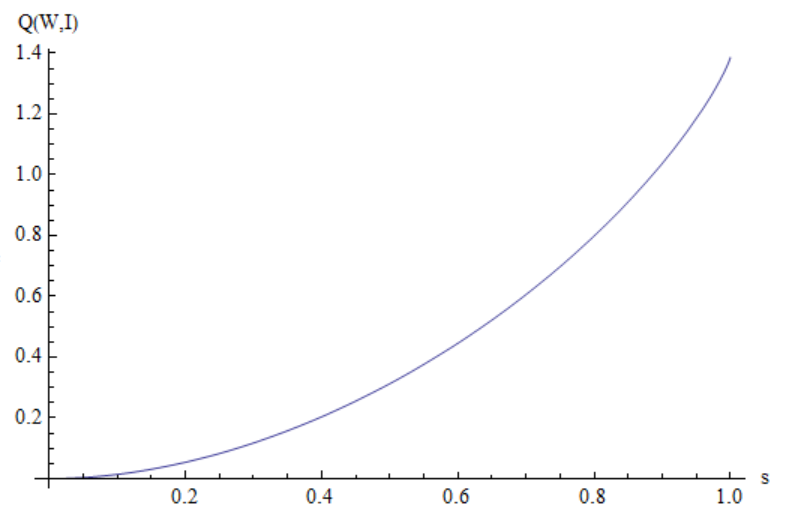
\includegraphics[scale=0.8]{figures/WIrelativecalc.png}
\caption{Plot of \eqref{hjreherjrie}.}
\label{figr5}
\end{center}
\end{figure}
\begin{equation}
Q(I_4 \| W)=\frac{1}{4} (-3 \log (1-s)-\log (3 s+1))
\label{dfsfsd}
\end{equation}
with its plot:
\begin{figure}[h]
\begin{center}
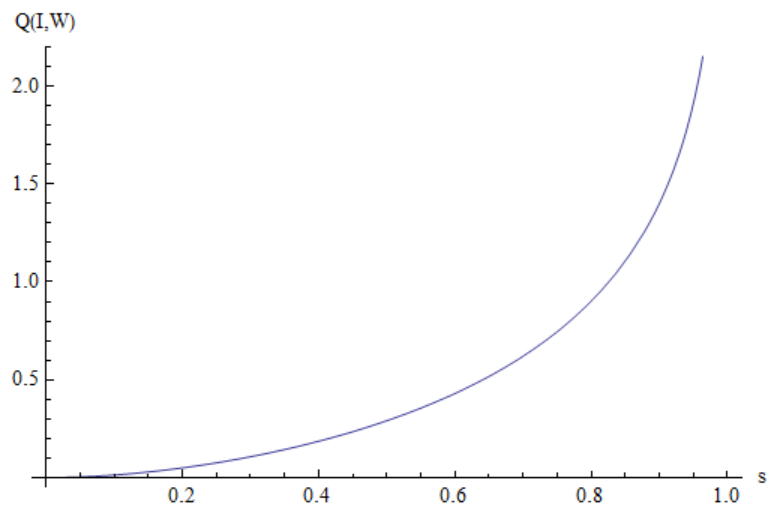
\includegraphics[scale=0.8]{figures/IWrelateivecalc.png}
\caption{The plot of \eqref{dfsfsd}.}
\label{figr6}
\end{center}
\end{figure}
\noindent
There is obvious asymmetry of the calculations however they have obvious qualitative commonalities.
\subsection{Mixed-Pure}
We now calculate the Relative entropy between the state $\sigma(\theta)$ of \eqref{sigmastate} and the Werner State \eqref{wernerstate} with $\ket{\Psi}=(\ket{00}+\ket{11})/\sqrt{2}$. We find that  
\begin{equation}
Q(\sigma\|W)=\frac{1}{2} \left(\log \left(\frac{16}{-3 s^2+2 s+1}\right)+\sin (2 \theta ) \log \left(\frac{1-s}{3 s+1}\right)\right)
\label{qentropy}
\end{equation}
with the plot:
\begin{figure}[H]
\begin{center}
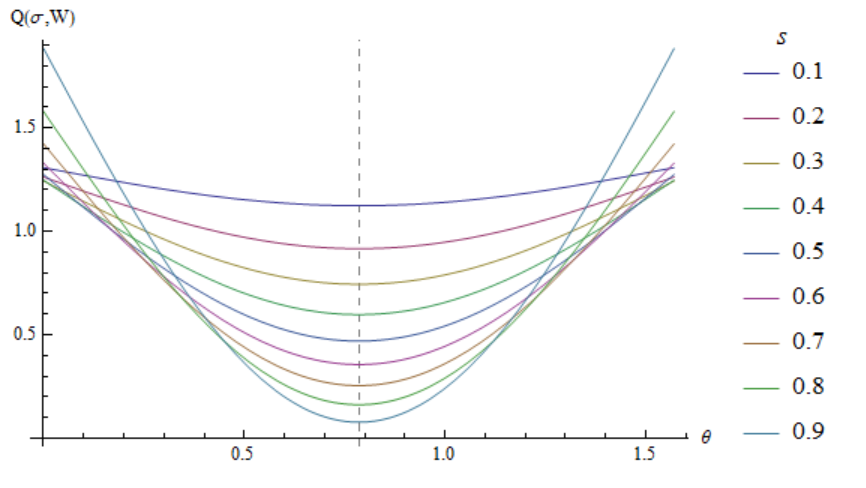
\includegraphics[scale=0.8]{figures/PureMixedRelativeEntropy.png}\caption{We can see that $Q(\sigma\|W)$ has an extremum for $s=0.5$ thus denoting that can be used as an entanglement measure.}
\label{figr7}
\end{center}
\end{figure}
\noindent
As we can see this measure of departure can detect the maximum entanglement of state $\sigma(\theta)$. This result might be useful in an experiment that can directly measure the quantum relative entropy.  We can easily check that $Q(W\|\sigma)$ diverges.

\chapter{Conclusions and further work}
\begin{itemize}
\item We have established that there can be experiments that measure entropies or entanglement measures directly. This means that without explicitly preparing the density matrix, we can deduce certain statistical properties of the system that may include entanglement. It is tempting to conjecture that if there can be designed an experiment that measures \ref{qentropy} directly, we can detect and quantify the entanglement of the pure state $\sigma(\theta)$. This claim is based on the plot \ref{figr7} combined with intuition from the conditional quantum entropy calculation of $\sigma(\theta)$ and the theory of entanglement entropy.
\item In \citep{wilde2013quantum} is proven for the quantum relative entropy that:
\begin{equation}
D(\rho \| \sigma)=\lim _{\varepsilon \to 0^{+}} D(\rho \| \sigma+\varepsilon I)
\end{equation}
Thus using a function $G(\varepsilon ;x)=x+\varepsilon$ different than ours for the matrix generalization, and taking the limit to zero. Since different functions $G(\varepsilon;x)$ can be used to heuristically determine the quantum relative entropy some questions rise. What is the class of functions that can be used in these calculations? Can we generally find the conditions needed? Are there any advantages and disadvantages among them? In addition, other functions withing relative entropy definitions like $g-relative$(\citep{holevo2012quantum}) or $f-relative$(\citep{hayashi2016quantum}) require further investigation regarding their connection with the class of functions $G(\epsilon;x)$.
\item Figures \ref{figuridion3d},\ref{figuridiont2},\ref{figuraki6},\ref{figr1},\ref{figr3},\ref{figr4},\ref{figr5},\ref{figr6},\ref{figr7} could not be found in the literature. I stand in the entanglement limit value plots in the Werner conditional entropy calculations, which demonstrate that for larger $q$'s and $a$'s we have smaller values of the conditional entropy. We are not aware of a general proof of this property. Thus raises the question for the generality of this result.
\end{itemize}
%\section{Further work}
%\begin{itemize}
%\item analytical proof of G and other functions
%\end{itemize}
\appendix
\chapter{Mathematica Code}
This is most of the notebook used for the calculations in the thesis. There are some function that are not defined here but there will become available on \href{https://github.com/jmstf94}{github}.
\label{appendix:code}
\section{Basics}
\begin{verbatim}
The first line makes mathematica arrays look like matrices at the outputs. 

The rest is a function that traces out a subsystem of quDits from a N-quDit system.
dTraceSystem has 3 arguments, the density matrix \[Rho], 
the list of qudits to trace out, 
e.g. {2, 3} and the dimension d of the qudits. This code was taken from the 
Wolfram Library Archive and it is called "Partial Trace of a MultiquDit System" 
by Mark Tame.
(https://library.wolfram.com/infocenter/MathSource/8763/)

ClearAll["Global`*"]
$PrePrint = If[MatrixQ[#], MatrixForm[#], #] &;
SwapParts[expr_, pos1_, pos2_] := 
 ReplacePart[#, #, {pos1, pos2}, {pos2, pos1}] &[expr]
dTraceSystem[D_, s_, dimen_] := (
  
  Qudits = Reverse[Sort[s]];
  TrkM = D;
  dim = dimen;
  
  z = (Dimensions[Qudits][[1]] + 1);
  
  For[q = 1, q < z, q++,
   n = Log[dim, (Dimensions[TrkM][[1]])];
   M = TrkM;
   k = Qudits[[q]];
   If[k == n,
    TrkM = {};
    For[p = 1, p < dim^n + 1, p = p + dim,
     TrkM = Append[TrkM, \!\(
\*UnderoverscriptBox[\(\[Sum]\), \(h = 0\), \(dim - 1\)]\(Take[
          M[\([\)\(p + h, All\)\(]\)], {1 + h, 
\*SuperscriptBox[\(dim\), \(n\)], dim}]\)\)];
      ],
    
    For[j = 0, j < (n - k), j++,
     b = {0};
     For[i = 1, i < dim^n + 1, i++,
      If[IntegerDigits[i - 1, dim, n][[n]] != 
         IntegerDigits[i - 1, dim, n][[n - j - 1]] && 
        Count[b, i]  == 0, 
       b = 
        Append[b, (FromDigits[
            
            SwapParts[(IntegerDigits[i - 1, dim, n]), {n}, {n - j - 
               1}], dim] + 1)];
       c = Range[dim^n];
       perm = 
        SwapParts[
         c, {i}, {(FromDigits[
             SwapParts[(IntegerDigits[i - 1, dim, n]), {n}, {n - j - 
                1}], dim] + 1)}];
       M = M[[perm, perm]];
        ]    
      ];
        ];
    
    TrkM = {};
    For[p = 1, p < dim^n + 1, p = p + dim,
     TrkM = Append[TrkM, \!\(
\*UnderoverscriptBox[\(\[Sum]\), \(h = 0\), \(dim - 1\)]\(Take[
          M[\([\)\(p + h, All\)\(]\)], {1 + h, 
\*SuperscriptBox[\(dim\), \(n\)], dim}]\)\)];
     ]
    ]
   ]
  
  ; Return[TrkM])
\end{verbatim}
\section{von Neumann I}
\begin{verbatim}
psi = (1/Sqrt[2])*{{0}, {1}, {-I}, {0}}
rho = KroneckerProduct[psi1, ConjugateTranspose[psi1]]
{vals, vecs} = Eigensystem[rho1]
M = Transpose[vecs1]
Det[M1]
Inverse[M]
DG = DiagonalMatrix[vals]
M.DG.Inverse[M] == rho;
F[x_] := Piecewise[{{x*Log[x], x > 0}, {0, x == 0}}, null];
FD = MatrixFunction[F, DG]
-Tr[M.FD.Inverse[M]]
\end{verbatim}
\section{von Neumann II}
\begin{verbatim}
$Assumptions = s \[Element] Reals && 0 < s < 1;
rho = Refine[{{s, 0}, {0, 1 - s}}]
{vals, vecs} = Refine[Eigensystem[rho]]
F[x_] := Piecewise[{{x*Log[x], x > 0}, {0, x == 0}}, null];
FD = Refine[MatrixFunction[F, rho]]
L = -Tr[FD]
Plot[L, {s, 0, 1}, AxesLabel -> {"s", "S (\[Rho])" }]
\end{verbatim}
\section{Renyi I}
\begin{verbatim}
$Assumptions = \[Alpha] \[Element] Reals && \[Alpha] > 
    0 && \[Alpha] != 1;
psi = (1/Sqrt[2])*{{0}, {1}, {-I}, {0}}
rho = KroneckerProduct[psi, ConjugateTranspose[psi]]
{vals, vecs} = Eigensystem[rho]
M = Transpose[vecs]
Det[M]
Inverse[M]
DG = DiagonalMatrix[vals]
M.DG.Inverse[M] == rho
F[x_] := x^\[Alpha];
matrixtrans = Refine[MatrixFunction[F, DG]]
matrixtransnext = M.matrixtrans.Inverse[M]
L = Tr[matrixtransnext]
Log[L]
\end{verbatim}
\section{Renyi II}
\begin{verbatim}
Clear[\[Alpha], s]
$Assumptions = \[Alpha] \[Element] Reals && \[Alpha] > 
    0 && \[Alpha] != 1;
$Assumptions = s \[Element] Reals && 0 < s < 1;
rho = {{s, 0}, {0, 1 - s}}
function[x_] := x^\[Alpha]
finalmatrix = MatrixFunction[function, rho]
L = Log[Tr[finalmatrix]]/(1 - \[Alpha])
Plot[Evaluate@Table[L, {\[Alpha], 0.1, 4, 0.4}], {s, 0, 1}, 
 PlotLegends -> 
  LineLegend[Table[\[Alpha], {\[Alpha], 0.1, 4, 0.4}], 
   LegendLabel -> \[Alpha]], AxesLabel -> {"s", "R(\[Alpha];\[Rho])"}]
Plot3D[L, {s, 0, 1}, {\[Alpha], 0, 15}, 
 AxesLabel -> {"s", "\[Alpha]", "R"}]
\end{verbatim}
\section{Tsallis I}
\begin{verbatim}
Clear[q];
$Assumptions = q \[Element] Reals && q > 0 && q != 1;
psi = (1/Sqrt[2])*{{0}, {1}, {-I}, {0}};
rho = KroneckerProduct[psi, ConjugateTranspose[psi]];
{vals, vecs} = Eigensystem[rho]
M = Transpose[vecs]
Det[M]
Inverse[M]
DG = DiagonalMatrix[vals]
M.DG.Inverse[M] == rho
t[x_] := x^q;
FD = Simplify[MatrixFunction[t, DG]]
trace = Tr[M.FD.Inverse[M]]
(trace - 1)/(1 - q)
\end{verbatim}
\section{Tsallis II}
\begin{verbatim}
Clear[q, s]
$Assumptions = q \[Element] Reals && q > 0 && q != 1;
$Assumptions = s \[Element] Reals && 0 < s < 1;
rho = {{s, 0}, {0, 1 - s}}
function[x_] := x^q
matr = MatrixFunction[function, rho]
L = ((Tr[matr]) - 1)/(1 - q)
Plot[Evaluate@Table[L, {q, 0.1, 4, 0.4}], {s, 0, 1}, 
 PlotLegends -> 
  LineLegend[Table[q, {q, 0.1, 4, 0.4}], LegendLabel -> q], 
 AxesLabel -> {"s", "T(q;\[Rho])"}]
Plot3D[L8, {s, 0, 1}, {q, 0, 15}, AxesLabel -> {"s", "q", "T"}]
\end{verbatim}
\section{Conditional}
\begin{verbatim}
Clear[\[Theta]]
$Assumptions = \[Theta] \[Element] Reals && 0 < \[Theta] < \[Pi]/2;
chi = {{Cos[\[Theta]]}, {0}, {0}, {Sin[\[Theta]]}}
sigma = Refine[KroneckerProduct[chi, ConjugateTranspose[chi]]]
{values, vecs} = Eigensystem[sigma]
M = Simplify[Transpose[vecs]]
FullSimplify[Det[M]]
Minv = Simplify[Inverse[M]]
diag = DiagonalMatrix[values]
sigma == M.diag.Minv
sigmaA = dTraceSystem[sigma, {2}, 2]
F[x_] := x*Log[x];
L = MatrixFunction[F, sigmaA]
FullSimplify[L3 = Tr[L]]
Plot[L3, {\[Theta], 0, \[Pi]/2}, AxesLabel -> {"\[Theta]", "S(A|B)"}]
Refine[L3, \[Theta] == \[Pi]/4]
\end{verbatim}
\section{Werner von Neumann}
\begin{verbatim}
$Assumptions = s \[Element] Reals && 0 < s < 1;
WernerState = {{(1 + s)/4, 0, 0, s/2}, {0, ((1 - s)/4), 0, 0}, {0, 
    0, (1 - s)/4, 0}, {s/2, 0, 0, (1 + s)/4}};
{Wvals, Wvecs} = Eigensystem[WernerState];
Mw = Refine[Transpose[Wvecs]];
Det[Mw];
Inverse[Mw];
DGw = Refine[DiagonalMatrix[Wvals]];
WernerState == Simplify[Mw.DG.Inverse[Mw]];
Fw[x_] := Piecewise[{{x*Log[x], x > 0}, {0, x == 0}}, null];
FDw = Refine[MatrixFunction[Fw, DGw]];

Simplify[-Tr[Mw.FDw.Inverse[Mw]]] == Simplify[vonNeumann[WernerState]];
Simplify[vonNeumann[WernerState]];
WernerStateA = Simplify[dTraceSystem[WernerState, {2}, 2]];
CSofWerner = vonNeumann[WernerState] - vonNeumann[WernerStateA]
Entanglementsvalue = N[Refine[CSofWerner, s == 1/3]];
N[Refine[vonNeumann[WernerStateA], s == 1/3]];
zerocondwerner = s /. FindRoot[CSofWerner, {s, 0.7}]

plot1 = Plot[CSofWerner, {s, 0, 1}, AxesLabel -> {"s", "S(B|A)"}, 
  GridLines -> {{{1/3, Dashed}}, {{Entanglementsvalue, Dashed}}}, 
  Epilog -> {{Blue, PointSize@Large, 
     Point[{1/3, Entanglementsvalue}]}, {Red, PointSize@Large, 
     Point[{zerocondwerner, 0}]}}]
\end{verbatim}
\section{Werner Tsallis}
\begin{verbatim}
Clear[s, x, q];
$Assumptions = s \[Element] Reals && 0 < s < 1;
WernerState = {{(1 + s)/4, 0, 0, s/2}, {0, ((1 - s)/4), 0, 0}, {0, 
    0, (1 - s)/4, 0}, {s/2, 0, 0, (1 + s)/4}};
WernerStateA = Simplify[dTraceSystem[WernerState, {2}, 2]];

{valsT, vecsT} = Refine[Eigensystem[WernerState]];
MT = Refine[Transpose[vecsT]];
Inverse[MT];
DGT = Refine[DiagonalMatrix[valsT]];
FT[y_] := Piecewise[{{y^x, y >= 0}}, null];
FDT = Refine[MatrixFunction[FT, DGT]];
MT.FDT.Inverse[MT];

Firstterm = (Tr[MT.FDT.Inverse[MT]] - 1)/(1 - x);

FDT2 = Refine[MatrixFunction[FT, WernerStateA]];
Secondterm = (Tr[FDT2] - 1)/(1 - x);
ResultingT = 
 Simplify[(Firstterm - Secondterm)/(1 + (1 - x)*Secondterm)]
Plot3D[ResultingT, {x, 0, 3}, {s, 0, 1}]

examplidionT1 = Refine[ResultingT, x == 0.3];
root1 = s /. FindRoot[examplidionT1, {s, 0.9}];
examplidionT2 = Refine[ResultingT, x == 0.9];
root2 = s /. FindRoot[examplidionT2, {s, 0.9}];
examplidionT3 = Refine[ResultingT, x == 1.5];
root3 = s /. FindRoot[examplidionT3, {s, 0.9}];
examplidionT4 = Refine[ResultingT, x == 2.1];
root4 = s /. FindRoot[examplidionT4, {s, 0.9}];
examplidionT5 = Refine[ResultingT, x == 2.7];
root5 = s /. FindRoot[examplidionT5, {s, 0.9}];
examplidionT6 = Refine[ResultingT, x == 3.3];
root6 = s /. FindRoot[examplidionT6, {s, 0.9}];
examplidionT7 = Refine[ResultingT, x == 3.9];
root7 = s /. FindRoot[examplidionT7, {s, 0.9}];

Root1 = examplidionT1 /. s -> 1/3;
Root2 = examplidionT2 /. s -> 1/3;
Root3 = examplidionT3 /. s -> 1/3;
Root4 = examplidionT4 /. s -> 1/3;
Root5 = examplidionT5 /. s -> 1/3;
Root6 = examplidionT6 /. s -> 1/3;
Root7 = examplidionT7 /. s -> 1/3;

Plot[Evaluate@Table[ResultingT, {x, 0.3, 4, 0.6}], {s, 0, 1}, 
 PlotLegends -> 
  LineLegend[Table[x, {x, 0.3, 4, 0.6}], LegendLabel -> x], 
 AxesLabel -> {"s", "T(B|A)"}, 
 GridLines -> {{{1/3, Dashed}}, {{Root1, Dashed}}}, 
 Epilog -> {{Red, PointSize[Large], Point[{1/3, Root1}]}, {Blue, 
    PointSize[Large], Point[{root1, 0}]}}]
EntanglementLimitValueT = Refine[ResultingT, s == 1/3];
Plot[EntanglementLimitValueT, {x, 0, 50}]
\end{verbatim}
\section{Werner Renyi}
\begin{verbatim}
Clear[\[Alpha], s]
$Assumptions = s \[Element] Reals && 0 < s < 1;
WernerState = {{(1 + s)/4, 0, 0, s/2}, {0, ((1 - s)/4), 0, 0}, {0, 
    0, (1 - s)/4, 0}, {s/2, 0, 0, (1 + s)/4}};
WernerStateA = Simplify[dTraceSystem[WernerState, {2}, 2]];
CRofWerner = 
  FullSimplify[
   Renyi[WernerState, \[Alpha]] - Renyi[WernerStateA, \[Alpha]]];
Clear[\[Alpha]]
{valsR, vecsR} = Refine[Eigensystem[WernerState]];
MR = Refine[Transpose[vecsR]];
Inverse[MR];
DGR = Refine[DiagonalMatrix[valsR]];
FR[y_] := Piecewise[{{y^\[Alpha], y >= 0}}, null];
FDR = Refine[MatrixFunction[FR, DGR]];
FDR;
FtermR = Simplify[Log[Tr[MR.FDR.Inverse[MR]]]/(1 - \[Alpha])];
FDR = Refine[MatrixFunction[FR, WernerStateA]];
FDR;
StermR = Simplify[Log[Tr[FDR]]/(1 - \[Alpha])];
ttt = Simplify[FtermR - StermR];

examplidionR1 = Refine[CRofWerner, \[Alpha] == 0.3];
Rroot1 = s /. FindRoot[examplidionR1, {s, 0.9}];
Root1 = examplidionR1 /. s -> 1/3;

Plot[Evaluate@Table[ttt, {\[Alpha], 0.3, 4, 0.6}], {s, 0, 1}, 
 PlotLegends -> 
  LineLegend[Table[\[Alpha], {\[Alpha], 0.3, 4, 0.6}], 
   LegendLabel -> \[Alpha]], AxesLabel -> {"s", "R(\[Alpha];W)"}, 
 GridLines -> {{{1/3, Dashed}}, {{Root1, Dashed}}}, 
 Epilog -> {{Red, PointSize[Large], Point[{1/3, Root1}]}, {Blue, 
    PointSize[Large], Point[{Rroot1, 0}]}}]


examplidionS = Refine[CRofWerner, \[Alpha] == 0.3];
s /. FindRoot[examplidionS, {s, 0.9}];

EntanglementLimitValue = Refine[CRofWerner, s == 1/3]
Plot[EntanglementLimitValue, {\[Alpha], 0, 50}]
Plot3D[ttt, {\[Alpha], 0, 3}, {s, 0, 1}]
\end{verbatim}
\section{Relative I}
\begin{verbatim}
Clear[t, u, psi, rho]
$Assumptions = t \[Element] Reals && 0 < t < \[Pi]/2;
$Assumptions = u \[Element] Reals && 0 < u < \[Pi]/2;
psit = {{Cos[t]}, {0}, {0}, {Sin[t]}};
rhot = Refine[KroneckerProduct[psit, ConjugateTranspose[psit]], 
  t \[Element] Reals ]
psi = {{Cos[u]}, {0}, {0}, {Sin[u]}};
rho = Refine[KroneckerProduct[psi, ConjugateTranspose[psi]]]
Kappa[x_] := 
  Piecewise[{{Log[x], x > 0}, {\[CurlyEpsilon], x == 0}}, null];

{valst, vecst} = FullSimplify[Refine[Eigensystem[rhot]]]
Mt = FullSimplify[Refine[Transpose[vecst]]]
DGt = Refine[DiagonalMatrix[valst]]
InveMt = FullSimplify[Inverse[Mt]]

Mt.MatrixFunction[Kappa, DGt].InveMt
FullSimplify[Tr[rho.Simplify[MatrixFunction[Kappa, rhot]]]]

Mt.MatrixFunction[Kappa, DGt].InveMt /. t -> u
FullSimplify[Tr[rho.Simplify[MatrixFunction[Kappa, rhot]]]]
\end{verbatim}
\section{Relative II}
\begin{verbatim}
$Assumptions = s \[Element] Reals && 0 < s < 1;
WernerState = {{(1 + s)/4, 0, 0, s/2}, {0, ((1 - s)/4), 0, 0}, {0, 
    0, (1 - s)/4, 0}, {s/2, 0, 0, (1 + s)/4}};
psi1 = (1/Sqrt[2])*{{0}, {1}, {-I}, {0}};
rho1 = KroneckerProduct[psi1, ConjugateTranspose[psi1]];
WernerState2 = Simplify[(1 - s)*IdentityMatrix[4]/4 + s*rho1];
{Wvals, Wvecs} = Eigensystem[WernerState2];
Mw = Refine[Transpose[Wvecs]]
Inverse[Mw]
DGw = Refine[DiagonalMatrix[Wvals]]
WernerState2 == Simplify[Mw.DGw.Inverse[Mw]]

MaximallyMixed = IdentityMatrix[4]/4
testcase1 = RelativeEntropy[WernerState2, MaximallyMixed]
Plot[testcase1, {s, 0, 1}, AxesLabel -> {"s", "Q(W,I)"}]
testcase2 = RelativeEntropy[MaximallyMixed, WernerState2]
Plot[testcase2, {s, 0, 1}, AxesLabel -> {"s", "Q(I,W)"}]
\end{verbatim}
\section{Relative III}
\begin{verbatim}
Clear[s, \[Theta], chi, sigma, WernerState, WernerState2, chi3, \
sigma3, WernerState2]
$Assumptions = 
  s \[Element] Reals && 0 < s < 1 && \[Theta] \[Element] Reals && 
   0 < \[Theta] < \[Pi]/2;
WernerState = {{(1 + s)/4, 0, 0, s/2}, {0, ((1 - s)/4), 0, 0}, {0, 
    0, (1 - s)/4, 0}, {s/2, 0, 0, (1 + s)/4}};

chi = {{Cos[\[Theta]]}, {0}, {0}, {Sin[\[Theta]]}};
sigma = Refine[KroneckerProduct[chi, ConjugateTranspose[chi]]];

case = RelativeEntropy[sigma, WernerState]

Plot[Evaluate@Table[case, {s, 0.1, 0.9, 0.1}], {\[Theta], 0, \[Pi]/2},
  PlotLegends -> 
  LineLegend[Table[s, {s, 0.1, 0.9, 0.1}], LegendLabel -> s], 
 AxesLabel -> {"\[Theta]", "Q(\[Sigma],W)"}, 
 GridLines -> {{{\[Pi]/4, Dashed}}, None}]
\end{verbatim}
\bibliographystyle{abbrv}
\bibliography{bibliography/biblio}
\end{document}